% \iffalse meta-comment
%
% Copyright (C) \the\year by Joseph Pan <cs.wzpan@gmail.com>
% This file may be distributed and/or modified under the
% conditions of the LaTeX Project Public License, either
% version 1.2 of this license or (at your option) any later
% version. The latest version of this license is in:
%
% http://www.latex-project.org/lppl.txt
%
% and version 1.2 or later is part of all distributions of
% LaTeX version 1999/12/01 or later.
%
% \fi
% 
% \iffalse
% <package>\NeedsTeXFormat{LaTeX2e}[1999/12/01]
% <package>\ProvidesPackage{scnuthesis}
% <package>		[2012/3/1 v0.5 By Joseph Pan <cs.wzpan@gmail.com>]
%
%<*driver>
\ProvidesFile{scnuthesis.dtx}[2013/11/24 v0.6.3 SCNUThesis]
\documentclass[11pt]{ltxdoc}
\usepackage{scnux}
\EnableCrossrefs
\CodelineIndex
\RecordChanges
\graphicspath{{figures/}}
\begin{document}
  \DocInput{\jobname.dtx}
\end{document}
%</driver>
% \fi
% 
% \def\thuthesis{\textsc{Thu}\-\textsc{Thesis}}
% \def\nudtpaper{\textsc{Nudt}\textsc{Paper}}
% \def\scnuthesis{\textsc{SCNU}\-\textsc{Thesis}}  
%
% \CheckSum{1241}
%
% \CharacterTable
%  {Upper-case    \A\B\C\D\E\F\G\H\I\J\K\L\M\N\O\P\Q\R\S\T\U\V\W\X\Y\Z
%   Lower-case    \a\b\c\d\e\f\g\h\i\j\k\l\m\n\o\p\q\r\s\t\u\v\w\x\y\z
%   Digits        \0\1\2\3\4\5\6\7\8\9
%   Exclamation   \!     Double quote  \"     Hash (number) \#
%   Dollar        \$     Percent       \%     Ampersand     \&
%   Acute accent  \'     Left paren    \(     Right paren   \)
%   Asterisk      \*     Plus          \+     Comma         \,
%   Minus         \-     Point         \.     Solidus       \/
%   Colon         \:     Semicolon     \;     Less than     \<
%   Equals        \=     Greater than  \>     Question mark \?
%   Commercial at \@     Left bracket  \[     Backslash     \\
%   Right bracket \]     Circumflex    \^     Underscore    \_
%   Grave accent  \`     Left brace    \{     Vertical bar  \|
%   Right brace   \}     Tilde         \~}
%
% \changes{v0.5}{2012/02/20}{初始版本}
%
% \GetFileInfo{\jobname.dtx}
% 
% \DoNotIndex{\begin,\end,\begingroup,\endgroup}
% \DoNotIndex{\ifx,\ifdim,\ifnum,\ifcase,\else,\or,\fi}
% \DoNotIndex{\let,\def,\xdef,\newcommand,\renewcommand}
% \DoNotIndex{\expandafter,\csname,\endcsname,\relax,\protect}
% \DoNotIndex{\Huge,\huge,\LARGE,\Large,\large,\normalsize}
% \DoNotIndex{\small,\footnotesize,\scriptsize,\tiny}
% \DoNotIndex{\normalfont,\bfseries,\slshape,\interlinepenalty}
% \DoNotIndex{\hfil,\par,\hskip,\vskip,\vspace,\quad}
% \DoNotIndex{\centering,\raggedright}
% \DoNotIndex{\c@secnumdepth,\@startsection}
% \DoNotIndex{\ ,\@plus,\@minus,\p@,\z@,\@m,\@M,\@ne,\m@ne}
% \DoNotIndex{\@@par,\DeclareOperation,\RequirePackage,\LoadClass}
% \DoNotIndex{\AtBeginDocument,\AtEndDocument}
%
% \IndexPrologue{\section*{索引}%
%    \addcontentsline{toc}{section}{索~~~~引}}
% \GlossaryPrologue{\section*{修改记录}%
%    \addcontentsline{toc}{section}{修改记录}}
%
% \renewcommand{\abstractname}{摘~~要}
% \renewcommand{\contentsname}{目~~录}
%
% \title{\textsc{SCNUThesis:}\,\,华南师范大学学位论文\\\LaTeX{}模板使用手册}
% \author{潘伟洲 \\ \href{mailto:cs.wzpan@gmail.com}{\texttt{cs.wzpan@gmail.com}}} 
% \date{\fileversion\ (\filedate)}
%
% \maketitle
% \thispagestyle{empty}
%
% \begin{abstract}
% 本模板旨在提供规范的华南师范大学\LaTeX{}写作模板环境,
% 现支持硕士/博士学位论文格式。
% \vspace{2em}
% \end{abstract}
%
% \vspace{2cm}
% \def\abstractname{免责声明}
% \begin{abstract}\noindent
% \begin{enumerate}
% \item 本模板的发布遵守 \LaTeX{} Project Public License,使用前请认真阅读协议内容。
% \item 本模板参照华南师范大学学位论文的基本要求和书写格式。
% \item 华南师范大学对论文写作提供写作指南与官方\textbf{doc}模板,
% 本模板的出发点是方便大家使用专业的高效的论文书写工具,
% 其优点在于注重排版质量、命令规范、使用方便、更新及时,符合论文撰写说明。
% 但任何由于使用本模板而引起的论文格式审查问题均与本模板作者无关。
% \item 任何个人或组织均可以本模板为基础进行修改、扩展,生成新的专用模板,但请严格遵守
% \LaTeX{} Project Public License 协议。
% \item 欢迎提出修改意见。
% \end{enumerate}
% \end{abstract}
%
% \clearpage
% \tableofcontents
%
% \clearpage
% \pagenumbering{arabic}
% \pagestyle{mainpage}
%
% \changes{v0.5.1}{2011/02/23}{修复了pro版makefile的bug}
% \section{快速上手}
% 这部分是专门为那些想快速开始写论文的人准备的。
% \begin{description}
% \item[~安装\TeX~] 下载最新的\TeX{}live或者C\TeX{}并安装
% \item[~字体~] 用户需要具备\verb|simsun.ttf|, \verb|simhei.ttf|, \verb|simkai.ttf|,
% 上述字体都是windows自带的; 除此之外,在网上下载(或者C\TeX{}
% 论坛) ``Adobe Opentype 中文字体'',确保下载下来Adobe的四款OTF字体:
% 宋,黑,仿宋,楷体。Linux用户可将上述字体复制到\verb|/usr/share/fonts/TTF|下。
% \item[~试一试~] 解压缩下载的模板,双击makepdf.bat(祈祷一下),如果生成了
% \verb|thesis.pdf|$\rightarrow$
% \item[~开始写了~] 所有文件均采用UTF8编码,因此要保证你的\TeX{}编辑器
% (winedt, texworks, texmaker, vim, 记事本($\cdots{}$)等)支持这种编码,
% (经过一番搜索设置后)打开\verb|thesis.tex|,如果看到的是中文$\rightarrow$
% \item[~漫长的写作~] 手边准备着\LaTeX{}的常用帮助文档(数学,图表,引用等),
% 结合你喜欢的文献管理软件(JabRef等), 漫长的\texttt{编辑,编译,修改,编辑,
% 编译$\cdots$}过程之后,你终于写完了$\rightarrow$
% \item[~校订~] 经过老师师兄师弟师妹齐心协力校正之后,你所做的只是:
% 装订,上交$\rightarrow$
% \end{description}
% {\color{magenta} Done!}
%
% \section{模板介绍}
%
% \textsc{SCNUThesis} 旨在帮助并且推广\LaTeX{}在华南师范大学论文中的应用,
% 本文将尽可能帮助用户掌握\textsc{SCNUThesis}的安装方法,
% 如果仍旧有不清晰的地方可以参考样例文件或者
% 给作者发邮件\footnote{作者邮箱:\url{mailto:cs.wzpan@gmail.com}},感兴趣的同学可以帮忙维护模板,
% 希望同学们在使用后能够提出你们的修改意见。
% 该模板很大程度上参考了国防科技大学的NUDTpaper
% \footnote{主页:\url{http://nudtpaper.googlecode.com}},
% 以及清华的Thuthesis
% \footnote{主页:\url{https://github.com/xueruini/thuthesis}},
% 对此表示感谢。
%
% {\color{blue}\fs 温馨提示:模板的作用在于减轻论文写作过程中格式调整的时间,
% 其前提就是遵守模板的用法,不提倡手动更改格式。
% 否则即使使用了\textsc{SCNUThesis}也难以保证输出的论文符合学校规范。}
%
% 另外,如果觉得我的模板对你起到帮助,非常希望能够得到你的肯定,在致谢里感谢
% \textsc{SCNUThesis},顺便起到推广的作用。例如 Jiaxin Pan 同学在其论文中的致谢:
%
% \begin{center}
%     \begin{minipage}{.9\textwidth}
%       \begin{tcolorbox}[colback=blue!10,colframe=blue!20,arc=3mm]
%         \begin{flushleft}
%         \hspace{0.5em}{\scalefont{1.2}\textbf{\begin{Huge}\textquotedblleft\end{Huge}}}
%         \\ \vspace{-0.65cm}
%         \hspace{2em}感谢XXX师兄、XXX师兄、XX、XX、XX、XXX等同实验室师兄弟,
%         与他们的讨论与交流促进了我的科研工作,也丰富了我的研究生生活。\textcolor{blue}{感谢潘伟洲
%         同学提供的\LaTeX{}排版模版\textsc{SCNUThesis}。}
%         \end{flushleft}
%     \end{tcolorbox}
%     \end{minipage}
% \end{center}
%
% \section{安装}
% \label{sec:install}
%
% \subsection{下载}
% \textsc{SCNUThesis} 主页:\url{http://wzpan.github.io/scnuthesis/}。
% 模板的更新信息发布在 \href{http://blog.josephpan.net}{我的博客}
% 以及 \href{http://bbs.scnu.edu.cn}{陶园BBS论坛}。
%
% \scnuthesis{}的开发版本同样可以在 \textsc{Github} 上获得:
% \changes{v0.5.5}{2011/06/01}{改为使用Git来做版本控制}
% \begin{shell}
% $ git clone git@github.com:wzpan/scnuthesis.git
% \end{shell}
%
% \subsection{模板的组成部分}
% 下表列出了 \scnuthesis{} 的主要文件及其功能介绍:
%
% \begin{center}
%   \begin{longtable}{l|p{10cm}}
% \hline
% {\hei 文件(夹)} & {\hei 功能描述}\\\hline\hline
% \endfirsthead
% \hline
% {\hei 文件(夹)} & {\hei 功能描述}\\\hline\hline
% \endhead
% \endfoot
% \endlastfoot
% scnux.sty & 论文格式宏包\\
% scnuthesis.ins* & 模板驱动文件 \\
% scnuthesis.dtx* & 模板文档代码的混合文件\\
% scnuthesis.cls & 模板类文件\\
% scnuthesis.cfg & 模板配置文件\\
% thesis.bib & 参考文献样式文件\\
% \hline
% myscnu.sty & 在这里添加你自己的宏包 \\
% thesis.tex & 示例文档主文件\\
% ref/ & 示例文档参考文献目录\\
% data/ & 示例文档章节具体内容\\
% figures/ & 示例文档图片路径\\
% \textbf{scnuthesis.pdf} & 用户手册(本文档)\\
% \textbf{thesis.pdf} & 示例文档 \\
% \hline
%   \end{longtable}
% \end{center}
% 需要说明几点:1) scnuthesis.ins 和 scnuthesis.dtx 是模板的源代码文件,不是编译
% 论文必须的文件,因此只在pro版给出,给有需要定制这个模板的高级用户使用。2)
% scnuthesis.cls 和 scnuthesis.cfg 由 scnuthesis.ins 和 scnuthesis.dtx 生成,但为
% 了降低新手用户的使用难度,在basic版中已直接给出。3) 学习使用模板的最好的办法就
% 修改示例文件\emph{thesis.tex}.
%
% \subsection{准备工作}
% \label{sec:prepare}
% 本模板需要以下宏包,如果你使用的是\TeX{}live或C\TeX{}的最新版本,
% 这一步可以安全的忽略。
%
% \begin{center}
% \begin{minipage}{0.8\linewidth}\centering
% \begin{tabular}{*{6}{l}}\hline
%   xunicode & xltxtra &
%	xeCJK\footnote{\href{http://bbs.ctex.org/viewthread.php?tid=40232&extra=page%3D1}{xeCJK 下载页}} &
%	array & booktabs & longtable  \\
%   amsmath & amssymb & ntheorem &
%   indentfirst & paralist & txfonts \\
%	natbib & hyperref &  &
%   graphicx & subfig\footnote{版本要求:$\geq$2005/06/28 ver: 1.3} &
%   caption\footnote{版本要求:$\geq$2006/03/21 v3.0j} \\
% \hline
% \end{tabular}
% \end{minipage}
% \end{center}
%
% \subsection{\TeX{}系统的选择}
% 有网络环境的用户推荐安装\href{http://www.tug.org/texlive}{\TeX{}live},
% \href{http://miktex.org}{MiKTeX}或者\href{http://www.ctex.org}{C\TeX},
% 对于无网络环境的,推荐{\TeX{}live}或者C\TeX{}完整版,安装
% 过程很简单,一路下一步即可,但是需要\textbf{注意:}
%
% \begin{description}
% \item[~字体~] TTF选项默认调用Windows系统字体,其中楷体,仿宋需要安装Office; OTF选项需要
% Adobe的商业字体(可以使你的论文更加漂亮!),中文字体(宋,黑,仿宋,楷体)可以从
% \href{http://ishare.iask.sina.com.cn/f/23186570.html}{这里下载}。
% 英文字体使用系统自带。
% \item[~xeCJK~] 无网络环境中,C\TeX{}完整版和\TeX{}live最新版都包括了需要的xeCJK版本。
% \end{description}
%
% \subsection{安装模板}
% \label{sec:install-cls}
% 不关心实现细节的用户可以跳过这一节。
%
% {\hei 注:默认的发行版本已经包含了可以使用的模板环境,
% 包括编译好的cls以及论文样例源文件,
% 想快速上手的话,可以直接参看\verb|thesis.tex|,进行修改。
% 写作的过程就是将你的论文的内容放到data文件夹中,
% 图片放到\verb|figures|文件夹中,用\textsc{jabref} 修改 \verb|thesis.bib|即可。}
%
% 当用户需要编译生成自己的PDF版论文时,需要依次输入:
% \begin{shell}
% $ xelatex thesis     
% $ bibtex thesis
% $ xelatex thesis
% $ xelatex thesis
% \end{shell}
%
% 而为了简化用户使用,模板中针对Windows和Linux分别提供了两个快捷脚本文件:
% \begin{enumerate}
% \item \textbf{Windows}:双击执行\verb|makepdf.bat|,或者使用下面的命令:
% \begin{shell}
% > makepdf.bat        
% \end{shell}
% \item \textbf{Linux}:使用下面的命令:
% \changes{v0.5.5}{2011/06/01}{使用shell脚本取代Makefile}
% \changes{v0.5.7}{2013/04/28}{重新改回Makefile编译}
% \begin{shell}
% $ make
% \end{shell}
% 编译完如果需要清除一下中间文件,可以使用下面的命令:
% \begin{shell}
% $ make clean
% \end{shell}
% \end{enumerate}
%
% \textbf{注意}:前面的``>''或者``\$''都只是cmd和shell下的提示符,不需要手动输入。
%
% 完成后就会在当前目录下生成\verb|thesis.pdf|文件,就是排好版的论文,不过这时的
% 内容还是空的。现在,就要进入激动人心的写作过程了。
%
% \section{使用说明}
% \label{sec:how-to-use}
%
% 在开始之前,先问自己几个问题:
% \begin{enumerate}\addtolength{\itemsep}{-5pt}
% \item 我是不是已经掌握了 \LaTeX{} 基础知识?
% \item 我是不是认真地阅读了模板文档?
% \item 周围有没有同学可以帮我?
% \end{enumerate}
%
% 更推荐用户去阅读示例文档的源代码,改写会给你一个快速的开始。
%
% \subsection{模板选项}
% 研究生、博士生的毕业论文的编排格式大体相同,主要在封面有所区别。为了让用户在编
% 写论文的时候灵活选择封面、单双面等排版方式,本模板特别提供了几个模板选
% 项,用户在使用的时候只需要先指定好着几个模板选项,就可以生成最匹配的模板。
%
% 论文的第一句话是调用模板:
%
% \changes{v0.5.4}{2011/05/11}{听取了Jiaxin Pan的建议,增加了chapterhead选项,可以将章节标题设为页眉}
%
%    \begin{macrocode}
%<thesis>%1. 如果是研究生论文,常用的选项是:
%<thesis>% \documentclass[master,twoside,vista,ttf]{scnuthesis}
%<thesis>%2. 如果是博士生论文,常用的选项是:
%<thesis>% \documentclass[doctor,twoside,vista,ttf]{scnuthesis}
%<thesis>%3. 如果使用是Windows XP之前的Windows系列,或者使用从这个系列拷贝过来的字体,则需要将Vista选项去掉,如:
%<thesis>% \documentclass[master,twoside,ttf]{scnuthesis}
%<thesis>%4. 建议使用OTF字体获得较好的页面显示效果
%<thesis>%   OTF字体从网上获得,各个系统名称统一,不用加vista选项
%<thesis>%   如果你下载的是最新的(1201)OTF英文字体,建议修改scnuthesis.cls,使用PS Std
%<thesis>%   \documentclass[doctor,twoside,otf]{scnuthesis}
%<thesis>%5. 如果想生成盲评,传递anon即可,仍需修改个人成果部分
%<thesis>% \documentclass[master,otf,anon]{scnuthesis}
%<thesis>%6. 让章节标题作为页眉,可以使用chapterhead选项。如果和twoside一起使用,则奇数页页眉为章节标题,偶数页为文章标题。
%<thesis>% \documentclass[master,otf,twoside,chapterhead]{scnuthesis}
%<thesis>%
%    \end{macrocode}
%    \begin{macrocode}
%<*thesis>
\documentclass[master,vista,ttf,twoside]{scnuthesis}
\usepackage{myscnu}

%</thesis>
%    \end{macrocode}
%
% 模板的参数设置(开关)描述:
%
%\begin{description}
%\item[~master,doctor~]
% 硕士论文使用master,博士论文使用doctor。
%\item[~twoside~]
% 指定论文为单面打印还是双面打印,当使用\verb|twoside|选项之后,
% 论文会将章节开在奇数页右手边,
% 默认为\verb|openany|单面打印。
%\item[~ttf,otf~]
% 决定使用何种字体,TTF默认使用Windows自带的字体,而OTF则使用Adobe的字体(需要下载),
% TTF字体的优势是满足学校论文对于字体的要求,缺点是制作出来的PDF文件在浏览时可能发虚,
% 而OTF字体屏幕显示饱满,而且字体有很多选项可以方便\XeTeX{}排版。推荐使用\textbf{otf}
% 选项。
% \item[~vista~]使用\textsc{vista}、\textsc{Win 7}的用户当启用TTF字体时,系统默认
%   的楷体、仿宋名称是 KaiTi 和 FangSong,而不
%   是 KaiTi\_GB2312 和 FangSong\_GB2312,这里加入开关进行切换。
% \item[~chapterhead~]让章节标题作为页眉,默认不打开这个选项。如果和twoside一起结
%   合使用,则奇数页的页眉将被设置为章节标题,而偶数页的页眉则依然为文章标题。
%\item[~anon~]
% 是否为盲评版本,如需盲评,请加上anon。
%\end{description}
%
% 如果需要使用自己定义的命令、宏包,请放于\verb|myscnu.sty|中。
% 事实上,该文件中已经添加了很多有用的宏包和命令,你可以参照修改。
% 这些之所以没有放到模板中,一则为了简洁,二则赋予用户在格式之外更多的自由。
% 里面的宏包有:代码高亮、算法环境、向量命令等,请仔细查看。
%
% 样例文件默认的是硕士论文(master),双面打印(twoside),TTF字体(ttf)。
%
% \subsection{论文结构}
%
% 硕士/博士生论文的形式结构如下:
%
% \begin{center}
%   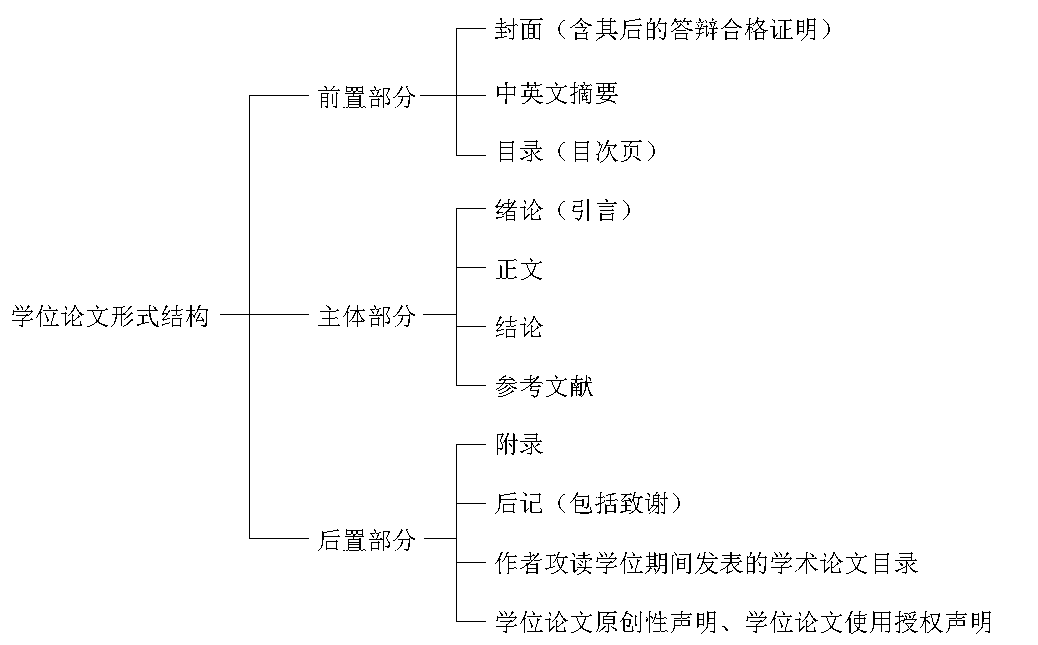
\includegraphics[width=\textwidth]{struct.pdf}
% \end{center}
% 
% 为了便于插入图形,模板中将图形文件单独放到一个目录中\verb|figure|中,论文正文各个
% 章节置于\verb|data|中;当然也以以\verb|chapter|为目录。看使用者的倾向了。
%
%    \begin{macrocode}
%<*thesis>
\begin{document}
\graphicspath{{figures/}}
%</thesis>
%    \end{macrocode}
%
% \subsection{前置部分}
% \subsubsection{封面}
% 封面上包括11项内容,具体包括:
% \begin{itemize}
% \item 论文封头:论文分类号、学校代码、密级、学号;
% \item 论文题目;
% \item 作者信息:作者姓名、专业、研究领域、学院、指导老师;
% \item 论文提交日期。
% \end{itemize}
%
% \begin{description}
% \item[~论文封头~]
% 包括论文分类号、学校代码、密级和学号。
%
% 其中,“论文分类号”按《中国图书资料分类法》的分类号填写;“密级”请根据情况
% 在“\textbf{无}、\textbf{秘密}、\textbf{机密}、\textbf{绝密}”中选择其一填写。
%
% \item[~论文题目~]
%
% 论文题目应能概括整个论文最重要的内容,应简明、恰当,一般不超过25个字(外语专
% 业的学位论文须有中文题目)。由于论文题目可能超过1行, 我们提供额外的一个命
% 令\verb|\displaytitle|用来填入在页眉等地方出现的单行的题目。
% \changes{v0.6}{2013/05/19}{作者基本信息迁移到 info.tex,导师职称和名字
% 分离} 
% 
% \end{description}
%
%    \begin{macrocode}
%<*thesis>
\classification{}
\university{10574}
\confidentiality{无}
\serialno{2011123456}
\title{华南师范大学硕士/博士学位论文\LaTeX{}模板使用手册}
\entitle{How to Use the \LaTeX{} Document Class for SCNU Dissertations}
\displaytitle{华南师范大学硕士/博士\\
  学位论文\LaTeX{}模板使用手册}
\author{张三}
\enauthor{San Zhang}
\subject{计算机应用技术}
\ensubject{Computer Applications Technology}
\researchfield{数字图像处理}
\school{计算机学院}
\supervisor{李四}
\ensupervisor{Si Li}
\protitle{教授}
\zhdate{\zhtoday}
 
%</thesis>
%    \end{macrocode}
%
% \subsubsection{中英文摘要}
%
% 摘要是学位论文内容概括性的简短陈述。它使读者可不阅读论文全文就能获得必要的信息。
% 摘要应具有独立性和自含性,即不阅读论文的全文,就能获得必要的信息。摘要中有数据、
% 有结论,是一篇完整的短文,可以独立使用,可以引用,可以用于工艺推广。摘要的内容
% 应包含与报告、论文同等量的主要信息,供读者确定有无必要阅读全文,也供文摘等二次
% 文献采用。摘要一般应说明研究工作目的、实验方法、结果和最终结论等,而重点是结果
% 和结论。要注意突出论文具有创新性的成果和新见解。硕士论文的中文摘要1000字左右。
% 博士论文的中文摘要1200字左右。外文摘要应是中文摘要的翻译,所表述的内容应与中文
% 摘要一致。
%
% 关键词:是为了文献标引工作从报告、论文中选取出来用以表示全文主题内容信息款目的
% 单词或术语。一般论文的关键词为3~8个。
%
% 模板中定义了相关环境\verb|\cabstract|以及\verb|\eabstract|来书写摘要,
% 以及\verb|\ckeywords|以及\verb|\ekeywords|来写关键字。
% 建议用户将摘要单独放在在\verb|abstract.tex|文件中,
% 在正文中\verb|\begin{cabstract}
华南师范大学是一所有着悠久历史和深厚人文底蕴的高等学府,学校地处中国改革开放之%
都——广州,深得岭南开放务实之精神,有着素朴的传统和良好的学风,七十多年来,学校坚%
持师范教育的特色,始终致力于培养人格健全、有思想、有能力、有社会责任感的优秀人才。%

在大学日益参与经济社会发展的新世纪,华南师范大学正以崭新的风貌、开阔的世界眼光,%
不断拓展大学的育人理念,创造良好的教学和包容的学术研究环境,营造丰富的校园文化,%
努力构建特色鲜明、开放式、综合性高水平教学研究型大学。%
\end{cabstract}
\ckeywords{华南师范大学;论文;模板}

\begin{eabstract}
  South China Normal University is an institution of higher education with a
  long history and a rich legacy. Situated in Guangzhou, the open metropolis in
  South China, South China Normal University is imbued with Lingnan's
  pioneering and pragmatic spirits. It has developed a tradition of elegant
  simplicity and fostered a strong learning environment. In the past seventy
  years or so, South China Normal University has preserved its characteristics
  of teacher education and has been devoted to cultivating talents with moral
  integrity, independent thinking, innovative ability and sense of social
  responsibility.

  In the new century in which the institutions of higher education are getting
  increasingly involved in the social and economic development, South China
  Normal University has adopted an international view on education. Having
  broadened its horizon on the key issue of cultivating talents, it has made its
  greatest efforts to create a congenial and harmonious environment for both
  teaching and academic research and has fostered a rich variety of campus
  culture. It aims to build itself into a high-level comprehensive teaching and
  research-oriented university with open distinctive features.
\end{eabstract}
\ekeywords{SCNU; thesis; template}

|即可。其格式为:
%
% \begin{example}
% \begin{cabstract}
% 中文摘要
% \end{cabstract}
% \ckeywords{关键字}
%
% \begin{eabstract}
% Abstract
% \end{eabstract}
% \ekeywords{Key}
% \end{example}
%
%<thesis>% 插入摘要,制作封面
%    \begin{macrocode}
%<*thesis>
\ifisanon{}\else{\maketitle}\fi
\frontmatter
\begin{cabstract}
华南师范大学是一所有着悠久历史和深厚人文底蕴的高等学府,学校地处中国改革开放之%
都——广州,深得岭南开放务实之精神,有着素朴的传统和良好的学风,七十多年来,学校坚%
持师范教育的特色,始终致力于培养人格健全、有思想、有能力、有社会责任感的优秀人才。%

在大学日益参与经济社会发展的新世纪,华南师范大学正以崭新的风貌、开阔的世界眼光,%
不断拓展大学的育人理念,创造良好的教学和包容的学术研究环境,营造丰富的校园文化,%
努力构建特色鲜明、开放式、综合性高水平教学研究型大学。%
\end{cabstract}
\ckeywords{华南师范大学;论文;模板}

\begin{eabstract}
  South China Normal University is an institution of higher education with a
  long history and a rich legacy. Situated in Guangzhou, the open metropolis in
  South China, South China Normal University is imbued with Lingnan's
  pioneering and pragmatic spirits. It has developed a tradition of elegant
  simplicity and fostered a strong learning environment. In the past seventy
  years or so, South China Normal University has preserved its characteristics
  of teacher education and has been devoted to cultivating talents with moral
  integrity, independent thinking, innovative ability and sense of social
  responsibility.

  In the new century in which the institutions of higher education are getting
  increasingly involved in the social and economic development, South China
  Normal University has adopted an international view on education. Having
  broadened its horizon on the key issue of cultivating talents, it has made its
  greatest efforts to create a congenial and harmonious environment for both
  teaching and academic research and has fostered a rich variety of campus
  culture. It aims to build itself into a high-level comprehensive teaching and
  research-oriented university with open distinctive features.
\end{eabstract}
\ekeywords{SCNU; thesis; template}



%</thesis>
%    \end{macrocode}
%
% \subsubsection{目录(目次页)}
% 完成摘要页后就是目录页。应能清楚表明各章节的层次关系。
%
% \changes{v0.5.4}{2011/05/11}{增加了表目录、图目录和符号列表} 
%<thesis>% 生成目录
%    \begin{macrocode}
%<*thesis>
\tableofcontents
\listoftables           % 如果要生成表目录
\listoffigures          % 如果要生成图目录

\renewcommand{\chapterlabel}{\denotationname} %设置页眉

\begin{denotation}

\item[SCNU] 华南师范大学 (South China Normal University)
\item[API] 应用程序编程接口  
\item[cluster] 集群
\item[graphic] 图形
\item[communication] 通信
\item[3D] 三维 (Three Dimemsion)
\item[BMP] 位图
\item[PNG] 便携式网络图形 (Portable Network Graphics)
\item[Watershed] 分水岭
\item[GUI] 图形用户界面 (Graphical User Interface)
\item[$E$] 能量
\item[$m$] 质量
\item[$c$] 光速
\item[$P$] 概率
\item[$T$] 时间
\item[$v$] 速度

\end{denotation}
 % 如果要生成符号列表

%</thesis>
%    \end{macrocode}
% \subsection{主体部分}
%
% 制作完前置部分后就是主体部分了,分别为:绪论、正文、结论和参考文献。
%
% \begin{description}
% \item[~绪论~] 
%   主要介绍本研究领域国内外研究现状,提出论文所要解决的问题以及该
%   研究工作在经济建设、科技进步和社会发展等方面的实用价值与理论意义。
% \item[~正文~] 
%   论文的核心部分,呈现研究工作的分析论证过程。正文的总体要求是:
%   实事求是、论据充分、逻辑清楚、层次分明、文字流畅、数据真实可靠。
% \item[~结论~] 
%   要求明确、精练、完整、准确,阐述论文创造性成果或新见解在本领域
%   的意义(应严格区分本人的研究成果与导师或其他人科研成果)。
% 由于绪论和结论在格式上和正文并没有不同,因此本模板并没有将这两个部分独立出来。
% 因此建议用户将绪论和结论作为正文的\emph{第一章}和\emph{最后一章}。
%
% 在写论文时可以在\verb|data/|文件夹中创建\verb|chap*.tex|文件,然后
% 在\verb|thesis.tex|中使用\verb|\input|语句引入进来。
%
% \item[~参考文献~] 
% 在\LaTeX{}下管理参考文献将极其方便,建议使用\verb|Jabref|生成条目,
% 用\verb|\cite|(其中\verb|upcite|是上标索引)索引即可。
% \verb|refs.bib|是你的参考文献名,可以根据需要换成你的。
%
% \end{description}
%
% \changes{v0.5.2}{2011/02/23}{修改了示例文档的一点细节}
% \changes{v0.5.3}{2011/02/23}{听取了Yin Chen的建议,添加了多行公式的示例}
% \changes{v0.5.3}{2011/02/23}{修改了示例文档中的少量错误标点}
% \changes{v0.5.5}{2011/06/01}{去掉了第一章中的表格和插图示例,统一在第二章中说
% 明}
% \changes{v0.5.7}{2013/04/28}{根据Jiawan Xu的反馈,解决了找不到参考文献样式的错
% 误}
% \changes{v0.6.1}{2013/05/20}{修正标点符号位于行首的问题,添加说明书相关教程}  
%<thesis>% 书写正文,可以根据需要增添章节。
%    \begin{macrocode}
%<*thesis>
\mainmatter
\chapter{绪论}

\section{本模板的意义}

\subsection{现有的学位论文模板的不足}
学位论文作为高校教学计划中的重要环节,对提高教学质量、培养学生综合应用能力具有十
分重要的意义。根据国家制定的《科学技术报告、学位论文和学术论文的编写格式》,华南
师范大学采用Microsoft Word等文字处理系统制作了相应的学位论文模板。然而,在应用这
些模板的过程中,却出现了几下几种问题:\cite{Maddage2009}
\begin{enumerate}
\item 无法自动处理图表、公式的序号、参考文献引用标号的变动,经常出现因疏忽而前后
  文体格式不一致的现象;
\item 无法实现论文的格式和内容的有效分离,导致模板的格式很容易被学生无意中修改,
  从而影响了学位论文规范化管理的质量;
\item 受制于Word版本的兼容性问题,在不同版本的文档之间常会有显示上的出入。
\end{enumerate}

\subsection{\LaTeX{}的特性}
\TeX{}作为一个功能强大的特别适合于排版科技文献和书籍的格式化排版程序,其具有以下
几点特性:
\begin{enumerate}
\item 强大的宏定义功能。\TeX{}是一种宏命令编程语言,能够处理非常复杂的排版任务,并生成高质量的输出;
\item 方便的自动编号功能。文章、书籍的章、节、段落以及公式、图表、参考文献、页码等均可自动编号;
\item 良好的通用性。\LaTeX{}几乎在所有的计算机操作系统平台上得到实现。\LaTeX{}的源文
  件可在不同的平台之间自由的交换,而得到的输出是完全相同的。
\end{enumerate}




\subsection{采用\LaTeX{}学位论文模板的意义}
采用\LaTeX{}学位论文模板将有以下几点意义:
\begin{enumerate}
\item 有效地解决以往的\verb|Word|模板中所存在的问题,有助于提高毕业生的学位论文的排版质量;
\item 有助于推动LaTeX在学生群体中的普及,学会使用\LaTeX{}来生成高质量的文档;
\item 课题最终的成果将完全开源,并在Google Code\footnote{项目主页:\url{http://code.google.com/p/scnuthesis/}}上公布。让更多爱好者研究学习,并不断完善,以适应日后的需求。
\end{enumerate}


\section{(1.2 题目)}
绪论内容

绪论内容

绪论内容

绪论内容

绪论内容

绪论内容

\section{(1.3 题目)}
绪论内容

绪论内容

绪论内容

绪论内容

绪论内容

绪论内容

\subsection{(1.3.1 题目)}
绪论内容

绪论内容

绪论内容

绪论内容

\subsection{(1.3.2 题目)}

绪论内容

绪论内容



\chapter{论文正文}
\label{chap:main}
本章将进入论文排版的正文
主要包括:字体段落,图片表格,公式定理,参考文献四部分。
版面将包括在\scnuthesis{}中使用到的所有格式,模板中自定义命令到或者特有的东西都将被一一介绍,
希望大家能看到对自己有用的东西,方便上手。

为了节省时间,这份说明的内容同样参考了国防科技大学的\nudtpaper{}模板~,在此表示感谢。

\section{字体段落}
\label{sec:font}

本节内容来自华南师范大学外部门户\footnote{外部门户主页:\url{http://www.scnu.edu.cn/}}。

华南师范大学始建于1933年,是一所学科门类齐全的国家“211 工程”重点建设大学和广东%
省省属重点大学。学校现有广州石牌、广州大学城和南海3个校区,占地面积共3079亩,%
校舍面积共 126万平方米。校园环境优美,景色怡人~,人文景观遍布,文化气息浓厚,为广%
大师生提供了良好的学习、工作和生活环境。

学校现有4个国家重点学科(含1个重点培育学科), 9个国家“211 工程”重点建设学%
科,2个广东省一级学科重点学科,11个广东省二级学科重点学科。有71个本科专业,有14个%
博士学位授权一级学科、90个博士学位授权点(未含2011年8月一级学科调整后新增的博士%
点)、1个博士专业学位授权点,33个硕士学位授权一级学科、174个硕士学位授权点(未%
含2011年8月一级学科调整后新增的硕士点)、10个硕士专业学位授权点,涉及到哲学、经济%
学、法学、教育学、文学、历史学、理学、工学、管理学、农学、医学等11个学科门%
类。 有12个博士后流动站。

学校拥有一批实力较强的实验室和科研基地。有教育部激光生命科学重点实验室、环境理论
化学重点实验室(省部共建)、教育部电化学储能材料与技术工程研究中心、卫生部(中医
药管理局)中医药与光子技术实验室、国家理科基础科学研究和教学人才培养基地、教育部
部省共建人文社科重点研究基地(心理应用研究中心)、国家体育总局重点研究基地(体育
社会科学研究基地),有7个广东省重点实验室(中心),6个广东省高校科研型重点实验
室,3个广东省高校产学研结合示范基地,6个广东省普通高校人文社会科学重点研究基
地,1个广东省高校工程技术研究中心。学校还拥有“物理学科基础课”、“信息传
播”~、“心理学”等3个国家级实验教学示范中心,7个广东省实验教学示范中心。此外,教
育部高校辅导员培训和研修基地、广东省普通高等学校师资培训中心~、广东省网络图书馆、
广东高校建筑规划设计院等机构均设在学校。

70 多年来,学校数易校名,几度迁徙,虽历经沧桑,却弦歌不辍。一代又一代华师人秉承勷
勤大学师范学院{\kai “研究高深学术,养成社会之专门人才”}的优良传统,承传南方大
学{\kai “忠诚团结,朴实虚心,勤劳勇敢,实事求是”}的革命精神~,践行{\kai “艰苦奋斗、严谨治
学、求实创新、为人师表”}的校训,筚路蓝缕,薪火相传,共同铸就了学校今天的繁荣与
发展。

华南师范大学历史上的名字包括:

\begin{itemize}
\item[楷体] {\kai 广州市立师范学校}
\item[黑体] {\hei 勷勤大学师范学院}
\item[隶书] {\li 勷勤大学教育学院}
\item[宋体] {\song 广东省立教育学院}
\item[仿宋] {\fs 广东省立文理学院}
\item[粗体] {\bfseries 广东省文理学院}
\item[斜体] {\itshape 华南师范学院}
\item[粗斜体] {\bfseries\itshape 广东师范学院}
\item[字体颜色] {\textcolor{red}{华南师范大学}}
\end{itemize}

上面这段内容使用了itemize列表环境,\LaTeX{}默认的列表环境会在条目之间插入
过多的行距,若用户需要紧凑的行距,可以使用compactitem环境。

下面测试英文字体:

Remember the \textsf{more} \textbf{font} {\bfseries\tiny you \sffamily use,
\Large the \scshape more \itshape beautiful \slshape your \footnotesize
document becomes.}

\begin{itemize}
\item[英文黑体] Typeset text in \textbf{bold} series
\item[英文斜体] Typeset text in \textit{italic} shape
\item[Roman字体] Typeset text in roman family
\item[Sans Serif字体] Typeset text in \textsf{sans serif} family
\item[typewriter字体] Typeset text in \texttt{typewriter} family
\end{itemize}

下面测试字号:
\begin{itemize}
\item[初号] {\chuhao 华南师范大学}
\item[小初] {\xiaochu 华南师范大学}
\item[一号] {\yihao 华南师范大学}
\item[小一] {\xiaoyi 华南师范大学}
\item[二号] {\erhao 华南师范大学}
\item[小二] {\xiaoer 华南师范大学}
\item[三号] {\sanhao 华南师范大学}
\item[小三] {\xiaosan 华南师范大学}
\item[四号] {\sihao 华南师范大学}
\item[小四] {\xiaosi 华南师范大学}
\item[五号] {\wuhao 华南师范大学}
\item[小五] {\xiaowu 华南师范大学}
\end{itemize}

\section{表格明细}
\label{sec:figure}
表格是书中的重要组成部分,这一章将从简单的表格讲起,到复杂的表格为止。

\subsection{基本表格}
\label{sec:basictable}

模板中关于表格的宏包有三个: \textsf{booktabs}、\textsf{array} 和
\textsf{longtabular},命令有一个 \verb|\hlinewd|。三线表建议使用\textsf{booktabs}中提供的,
包含toprule、midrule 和 bottomrule三条命令。
它们与\textsf{longtable} 能很好的配合使用。如果表格比较简单的话可以直接用命令
\verb|hlinewd{xpt}| 控制。下面来看一个表格:
\begin{table}[htb]
  \centering
  \begin{minipage}[t]{0.8\linewidth} % 如果想在表格中使用脚注,minipage是个不错的办法
  \caption[模板文件]{模板文件。如果表格的标题很长,那么在表格索引中就会很不美
    观,所以要像 chapter 那样在前面用中括号写一个简短的标题。这个标题会出现在索
    引中。}
  \label{tab:template-files}
    \begin{tabular*}{\linewidth}{lp{10cm}}
      \toprule[1.5pt]
      {\hei 文件名} & {\hei 描述} \\
      \midrule[1pt]
      scnuthesis.ins & \LaTeX{} 安装文件,docstrip\footnote{表格中的脚注} \\
      scnuthesis.dtx & 所有的一切都在这里面\footnote{再来一个}。\\
      scnuthesis.cls & 模板类文件。\\
      scnuthesis.cfg & 模板配置文。cls 和 cfg 由前两个文件生成。\\
      bstutf8.bst   & 参考文献 Bibtex 样式文件。\\
      myscnu.sty    & 常用的包和命令写在这里,减轻主文件的负担。\\
      \bottomrule[1.5pt]
    \end{tabular*}
  \end{minipage}
\end{table}

如果你不需要在表格中插入脚注,可以将minipage环境去掉。

表 \ref{tab:template-files} 列举了本模板主要文件及其功能。
请大家注意三线表中各条线对应的命令。这个例子还展示了如何在表格中正确使用脚注。
由于 \LaTeX{} 本身不支持在表格中使用 \verb|\footnote|,所以我们不得不将表格放在
小页中,而且最好将表格的宽度设置为小页的宽度,这样脚注看起来才更美观。

如果遇到表格内容自动调整的问题,可以有两种解决办法: 其一就是用\verb|tabular*|,在
两列之间全部插入空白,该方法存在的缺点是当只有两列需要自动调整时,若小页预留空间
过大,可能插入过多的\verb|fill|,导致不美观; 另外一种就是使用\verb|tabularx|自动
调整了,需要定制一个\textbf{Z}环境,在新版本中,该命令已添加到\verb|myscnu.sty|中。
下面是这两个方法实现的对比,各位可以仔细对比一下,推荐使用后者。

\begin{table}[htbp]
\centering
\begin{minipage}[t]{0.9\linewidth}
\caption{Reed Solomon码的典型应用}
\label{tab:RSused}
\begin{tabular*}{\linewidth}{c @{\extracolsep{\fill}} c}
\toprule[1.5pt]
{\hei 应用领域} & {\hei 编码方案}\\
\midrule[1pt]
磁盘驱动器 & RS(32,28,5)码 \footnote{码长为32、维数为28、最小距离为5} \\
CD & 交叉交织RS码(CIRC) \\
DVD & RS(208,192,17)码、RS(182,172,11)码 \\
光纤通信 & RS(255,229,17)码 \\
\bottomrule[1.5pt]
\end{tabular*}
\end{minipage}
\end{table}

\begin{table}[htbp]
\centering
\begin{minipage}[t]{0.9\linewidth}
\caption{Reed Solomon码的典型应用}
\label{tab:RSuse}
\begin{tabularx}{\linewidth}{cZ}
\toprule[1.5pt]
{\hei 应用领域} & {\hei 编码方案}\\
\midrule[1pt]
磁盘驱动器 & RS(32,28,5)码 \footnote{码长为32、维数为28、最小距离为5} \\
CD & 交叉交织RS码(CIRC) \\
DVD & RS(208,192,17)码、RS(182,172,11)码 \\
光纤通信 & RS(255,229,17)码 \\
\bottomrule[1.5pt]
\end{tabularx}
\end{minipage}
\end{table}

\subsection{复杂表格}
\label{sec:complicatedtable}

我们经常会在表格下方标注数据来源,或者对表格里面的条目进行解释。前面的脚注是一种
不错的方法,如果你不喜欢脚注。那么完全可以在表格后面自己写注释,比如表~\ref{tab:tabexamp1}。
\begin{table}[htbp]
  \centering
  \caption{复杂表格示例 1}
  \label{tab:tabexamp1}
  \begin{minipage}[t]{0.8\textwidth} 
    \begin{tabularx}{\linewidth}{|l|X|X|X|X|}
      \hline
      \multirow{2}*{\backslashbox{x}{y}}  & \multicolumn{2}{c|}{First Half} & \multicolumn{2}{c|}{Second Half}\\
      \cline{2-5}
      & 1st Qtr &2nd Qtr&3rd Qtr&4th Qtr \\ 
      \hline
      East$^{*}$ &   20.4&   27.4&   90&     20.4 \\
      West$^{**}$ &   30.6 &   38.6 &   34.6 &  31.6 \\ 
      \hline
    \end{tabularx}\\[2pt]
    \footnotesize
    *:东部\\
    **:西部
  \end{minipage}
\end{table}

此外,表~\ref{tab:tabexamp1} 同时还演示了另外两个功能:1)通过 \textsf{tabularx} 的
 \texttt{|X|} 扩展实现表格自动放大;2)通过命令 \verb|\backslashbox| 在表头部分
插入反斜线。

为了使我们的例子更接近实际情况,我会在必要的时候插入一些“无关”文字,以免太多图
表同时出现,导致排版效果不太理想。

学校七十余载薪火相传,名师荟萃,著名的教育家罗浚、汪德亮,五四新诗开创者之一康白
情,古代文学家李镜池,古汉语学家吴三立,历史学家王越,逻辑学家李匡武,心理学家阮
镜清,教育学家叶佩华、朱勃,数学家叶述武,物理学家黄友谋、刘颂豪,著名体育教育家
袁浚等众多名家、名师先后在此执教。该校虽数度易名、几经迁徙,但一代又一代华师人秉
承勷勤大学师范学院``研究高深学术,养成社会之专门人才''的优良传统,承传南方大
学``忠诚团结,实事求是''的革命精神,践行``艰苦奋斗、严谨治学、求实创新、为人师
表''的校训,不断推动学校事业向前发展。特别是改革开放以来,抓住科教兴国、人才强国
的发展机遇,凭借建设文化省、教育强省和国家``211工程''的强劲东风,形成了学校现在
跨越式发展的大好局面。

不可否认 \LaTeX{} 的表格功能没有想象中的那么强大,不过只要你足够认真,足够细致,那么
同样可以排出来非常复杂非常漂亮的表格。请参看表~\ref{tab:tabexamp2}。
\begin{table}[htbp]
  \centering\dawu[1.3]
  \caption{复杂表格示例 2}
  \label{tab:tabexamp2}
  \begin{tabular}[c]{|c|m{0.8in}|c|c|c|c|c|}\hline
    \multicolumn{2}{|c|}{Network Topology} & \# of nodes & 
    \multicolumn{3}{c|}{\# of clients} & Server \\\hline
    GT-ITM & Waxman Transit-Stub & 600 &
    \multirow{2}{2em}{2\%}& 
    \multirow{2}{2em}{10\%}& 
    \multirow{2}{2em}{50\%}& 
    \multirow{2}{1.2in}{Max. Connectivity}\\\cline{1-3}
    \multicolumn{2}{|c|}{Inet-2.1} & 6000 & & & &\\\hline
    \multirow{2}{1in}{Xue} & Rui  & Ni &\multicolumn{4}{c|}{\multirow{2}*{\scnuthesis}}\\\cline{2-3}
    & \multicolumn{2}{c|}{ABCDEF} &\multicolumn{4}{c|}{} \\\hline
\end{tabular}
\end{table}

\subsection{子表格与跨页表格}

浮动体的并排放置一般有两种情况:1)二者没有关系,为两个独立的浮动体;2)二者隶属
于同一个浮动体。对表格来说并排表格既可以像图~\ref{tab:parallel1}、图~\ref{tab:parallel2} 
使用小页环境,也可以如图~\ref{tab:subtable} 使用子表格来做。后面我们将讲解图的例子。
\begin{table}[htb]
\noindent\begin{minipage}{0.45\textwidth}
\centering
\caption{第一个并排子表格}
\label{tab:parallel1}
\begin{tabular}{p{2cm}p{2cm}}
\toprule[1.5pt]
111 & 222 \\\midrule[1pt]
222 & 333 \\\bottomrule[1.5pt]
\end{tabular}
\end{minipage}
\begin{minipage}{0.45\textwidth}
\centering
\caption{第二个并排子表格}
\label{tab:parallel2}
\begin{tabular}{p{2cm}p{2cm}}
\toprule[1.5pt]
111 & 222 \\\midrule[1pt]
222 & 333 \\\bottomrule[1.5pt]
\end{tabular}
\end{minipage}
\end{table}

学校教师队伍结构良好、水平较高,拥有一批在国内外具有一定影响的专家学者。现有教师
队伍 1900 多人,其中教授 400 多人,副教授 500 多人,博士、硕士研究生导师 800 多人,
具有博士、硕士学位和研究生学历的1500 多人。在师资队伍中,有中国科学院院士 7 人、
瑞典皇家科学院院士2人、“千人计划”入围者 1人、长江学者4人、获得国家杰出青年基金
项目资助者3人、“新世纪百千万人才”国家级人选 5人、国家级教学名师2 人、广东省领军
人才4人、珠江学者4人、广东省高等学校“千百十工程”国家级培养对象5人,拥有教育
部“长江学者与创新团队发展计划”创新团队 1个、广东省创新科研团队1个,并有国务院学
位委员会学科评议组成员 3 人、教育部高等学校教学指导委员会成员 12 人。

\begin{table}[htbp]
\centering
\caption{并排子表格}
\label{tab:subtable}
\subfloat[第一个子表格]{
\begin{tabular}{p{2cm}p{2cm}}
\toprule[1.5pt]
111 & 222 \\\midrule[1pt]
222 & 333 \\\bottomrule[1.5pt]
\end{tabular}}\hskip2cm
\subfloat[第二个子表格]{
\begin{tabular}{p{2cm}p{2cm}}
\toprule[1.5pt]
111 & 222 \\\midrule[1pt]
222 & 333 \\\bottomrule[1.5pt]
\end{tabular}}
\end{table}

如果您要排版的表格长度超过一页,那么推荐使用 \textsf{longtable} 或者 \textsf{supertabular} 
宏包,表~\ref{tab:performance} 就是 \textsf{longtable} 的简单示例。
\begin{longtable}[c]{c*{6}{r}}
\caption{实验数据}\label{tab:performance}\\
\toprule[1.5pt]
 测试程序 & \multicolumn{1}{c}{正常运行} & \multicolumn{1}{c}{同步}
& \multicolumn{1}{c}{检查点}   & \multicolumn{1}{c}{卷回恢复}
& \multicolumn{1}{c}{进程迁移} & \multicolumn{1}{c}{检查点} 	\\
& \multicolumn{1}{c}{时间 (s)} & \multicolumn{1}{c}{时间 (s)}
& \multicolumn{1}{c}{时间 (s)} & \multicolumn{1}{c}{时间 (s)}
& \multicolumn{1}{c}{时间 (s)} &  文件(KB)			\\
\midrule[1pt]%
\endfirsthead%

\multicolumn{7}{c}{续表~\thetable\hskip1em 实验数据}\\

\toprule[1.5pt]
 测试程序 & \multicolumn{1}{c}{正常运行} & \multicolumn{1}{c}{同步} 
& \multicolumn{1}{c}{检查点}   & \multicolumn{1}{c}{卷回恢复}
& \multicolumn{1}{c}{进程迁移} & \multicolumn{1}{c}{检查点} 	\\
& \multicolumn{1}{c}{时间 (s)} & \multicolumn{1}{c}{时间 (s)}
& \multicolumn{1}{c}{时间 (s)} & \multicolumn{1}{c}{时间 (s)}
& \multicolumn{1}{c}{时间 (s)} &  文件(KB)			\\
\midrule[1pt]%
\endhead%
\hline%

\multicolumn{7}{r}{续下页}%

\endfoot%
\endlastfoot%
CG.A.2 & 23.05   & 0.002 & 0.116 & 0.035 & 0.589 & 32491  \\
CG.A.4 & 15.06   & 0.003 & 0.067 & 0.021 & 0.351 & 18211  \\
CG.A.8 & 13.38   & 0.004 & 0.072 & 0.023 & 0.210 & 9890   \\
CG.B.2 & 867.45  & 0.002 & 0.864 & 0.232 & 3.256 & 228562 \\
CG.B.4 & 501.61  & 0.003 & 0.438 & 0.136 & 2.075 & 123862 \\
CG.B.8 & 384.65  & 0.004 & 0.457 & 0.108 & 1.235 & 63777  \\
MG.A.2 & 112.27  & 0.002 & 0.846 & 0.237 & 3.930 & 236473 \\
MG.A.4 & 59.84   & 0.003 & 0.442 & 0.128 & 2.070 & 123875 \\
MG.A.8 & 31.38   & 0.003 & 0.476 & 0.114 & 1.041 & 60627  \\
MG.B.2 & 526.28  & 0.002 & 0.821 & 0.238 & 4.176 & 236635 \\
MG.B.4 & 280.11  & 0.003 & 0.432 & 0.130 & 1.706 & 123793 \\
MG.B.8 & 148.29  & 0.003 & 0.442 & 0.116 & 0.893 & 60600  \\
LU.A.2 & 2116.54 & 0.002 & 0.110 & 0.030 & 0.532 & 28754  \\
LU.A.4 & 1102.50 & 0.002 & 0.069 & 0.017 & 0.255 & 14915  \\
LU.A.8 & 574.47  & 0.003 & 0.067 & 0.016 & 0.192 & 8655   \\
LU.B.2 & 9712.87 & 0.002 & 0.357 & 0.104 & 1.734 & 101975 \\
LU.B.4 & 4757.80 & 0.003 & 0.190 & 0.056 & 0.808 & 53522  \\
LU.B.8 & 2444.05 & 0.004 & 0.222 & 0.057 & 0.548 & 30134  \\
EP.A.2 & 123.81  & 0.002 & 0.010 & 0.003 & 0.074 & 1834   \\
EP.A.4 & 61.92   & 0.003 & 0.011 & 0.004 & 0.073 & 1743   \\
EP.A.8 & 31.06   & 0.004 & 0.017 & 0.005 & 0.073 & 1661   \\
EP.B.2 & 495.49  & 0.001 & 0.009 & 0.003 & 0.196 & 2011   \\
EP.B.4 & 247.69  & 0.002 & 0.012 & 0.004 & 0.122 & 1663   \\
EP.B.8 & 126.74  & 0.003 & 0.017 & 0.005 & 0.083 & 1656   \\
\bottomrule[1.5pt]
\end{longtable}

为了排版方便,这里要插入一些随机的文字,那就加上猩猩博客的东西吧: 
``越来越喜欢吃,自己做的川菜,每次做菜,都像是创作的过程,%
随心所欲; 发现家常菜真的很难做好,越是简单的菜,越是难以做好。
献上一个鱼香肉丝,让我跟随简单的脚步,creat出简约的菜品。''

\subsection{其它}
\label{sec:tableother}
有的同学不想让某个表格或者图片出现在索引里面,那么请使用命令 \verb|\caption*{}|,
这个命令不会给表格编号,也就是出来的只有标题文字而没有“表~XX”,“图~XX”,否则
索引里面序号不连续就显得不伦不类,这也是 \LaTeX{} 里星号命令默认的规则。

\section{绘图插图}

绘图工具分为 GUI 的和 CLI 两种。GUI即是所见即所得的绘图工具~,常见的包
括 Visio、Inkscape、CorelDraw、XFig(jFig)、WinFig、Tpx、Ipe、Dia等;CLI则是需要编
译后才能够得到图形的工具,比较流行的有 PGF/TikZ~、Asymptote、pstricks等。GUI 类绘
图工具比较易于上手,而 CLI 类绘图工具则能够画出更加精确的图形。关于各类绘图工具的
比较和使用方法~,推荐用户到C\TeX{}论坛{\url{http://bbs.ctex.org/}}以及China\TeX{}论坛
{\url{http://bbs.chinatex.org/forum.php}}上的相关板块进行更加深入的了解。

\subsection{插图}
\label{sec:graphs}

强烈推荐《\LaTeXe 插图指南》!关于子图形使用细节请参看\textsf{subfig}手册。 

\subsubsection{一个图形}
\label{sec:onefig}
一般图形都是处在浮动环境中。之所以称为浮动是指最终排版效果图形的位置不一定与源文
件中的位置对应,这也是刚使
用 \LaTeX{} 同学可能遇到的问题。如果要强制固定浮动图形的位置,请使用 \textsf{float} 宏包,
它提供了 \texttt{[H]} 参数,但是除非特别需要,不建议使用\texttt{[H]},
而是倾向于使用\texttt{[htbp]},给\LaTeX{}更多选择。比如图~\ref{fig:ipe}。
\begin{figure}[htbp] % use float package if you want it here
  \centering
  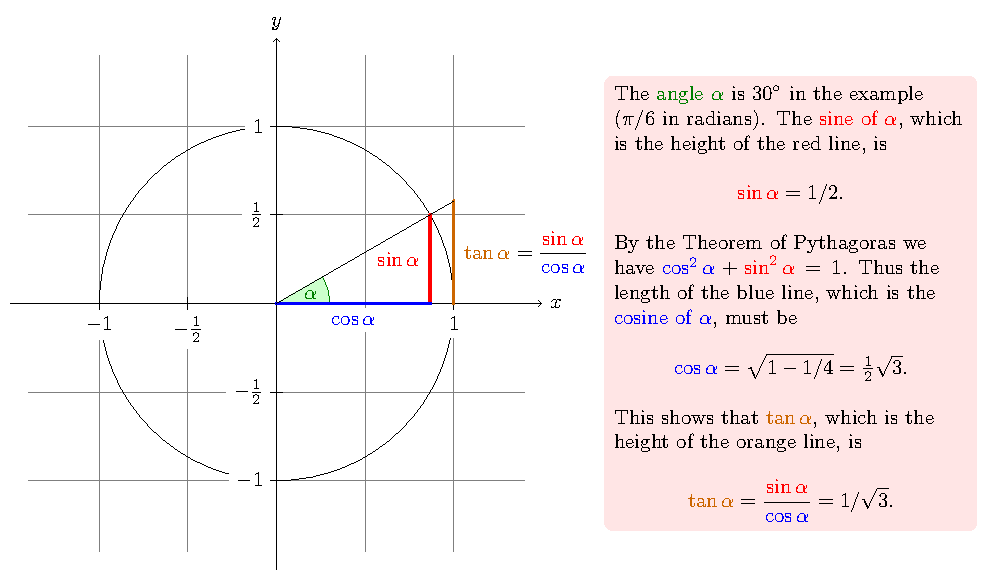
\includegraphics[width=\textwidth]{tikz}
  \caption{利用TikZ制图}
  \label{fig:ipe}
\end{figure}

大学之道,在明明德,在亲民,在止于至善。知止而后有定;定而后能静;静而后能安;安
而后能虑;虑而后能得。物有本末,事有终始。知所先后,则近道矣。古之欲明明德于天
下者,先治其国;欲治其国者,先齐其家;欲齐其家者~,先修其身;欲修其身者,先正其心;
欲正其心者,先诚其意;欲诚其意者~,先致其知;致知在格物。物格而后知至;知至而后
意诚;意诚而后心正;心正而后身修;身修而后家齐;家齐而后国治;国治而后天下
平。自天子以至于庶人,壹是皆以修身为本。其本乱而未治者 否矣。其所厚者薄,而其所
薄者厚,未之有也!

\hfill \pozhehao《大学》

\subsubsection{多个图形}
\label{sec:multifig}

如果多个图形相互独立,并不共用一个图形计数器,那么用 \verb|minipage| 或者
\verb|parbox| 就可以。否则,请参看图~\ref{fig:big1},它包含两个小图,分别是图~\ref{fig:subfig1} 
和图~\ref{fig:subfig2}。推荐使用 \verb|\subfloat|,不要再用
\verb|\subfigure| 和 \verb|\subtable|。
\begin{figure}[htb]
  \centering%
  \subfloat[第一个小图形]{%
    \label{fig:subfig1}
    
\includegraphics[height=2cm]{logo.jpg}}\hspace{4em}%
  \subfloat[第二个小图形。如果标题很长的话,它会自动换行,这个 caption 就是这样的例子]{%
    \label{fig:subfig2}
    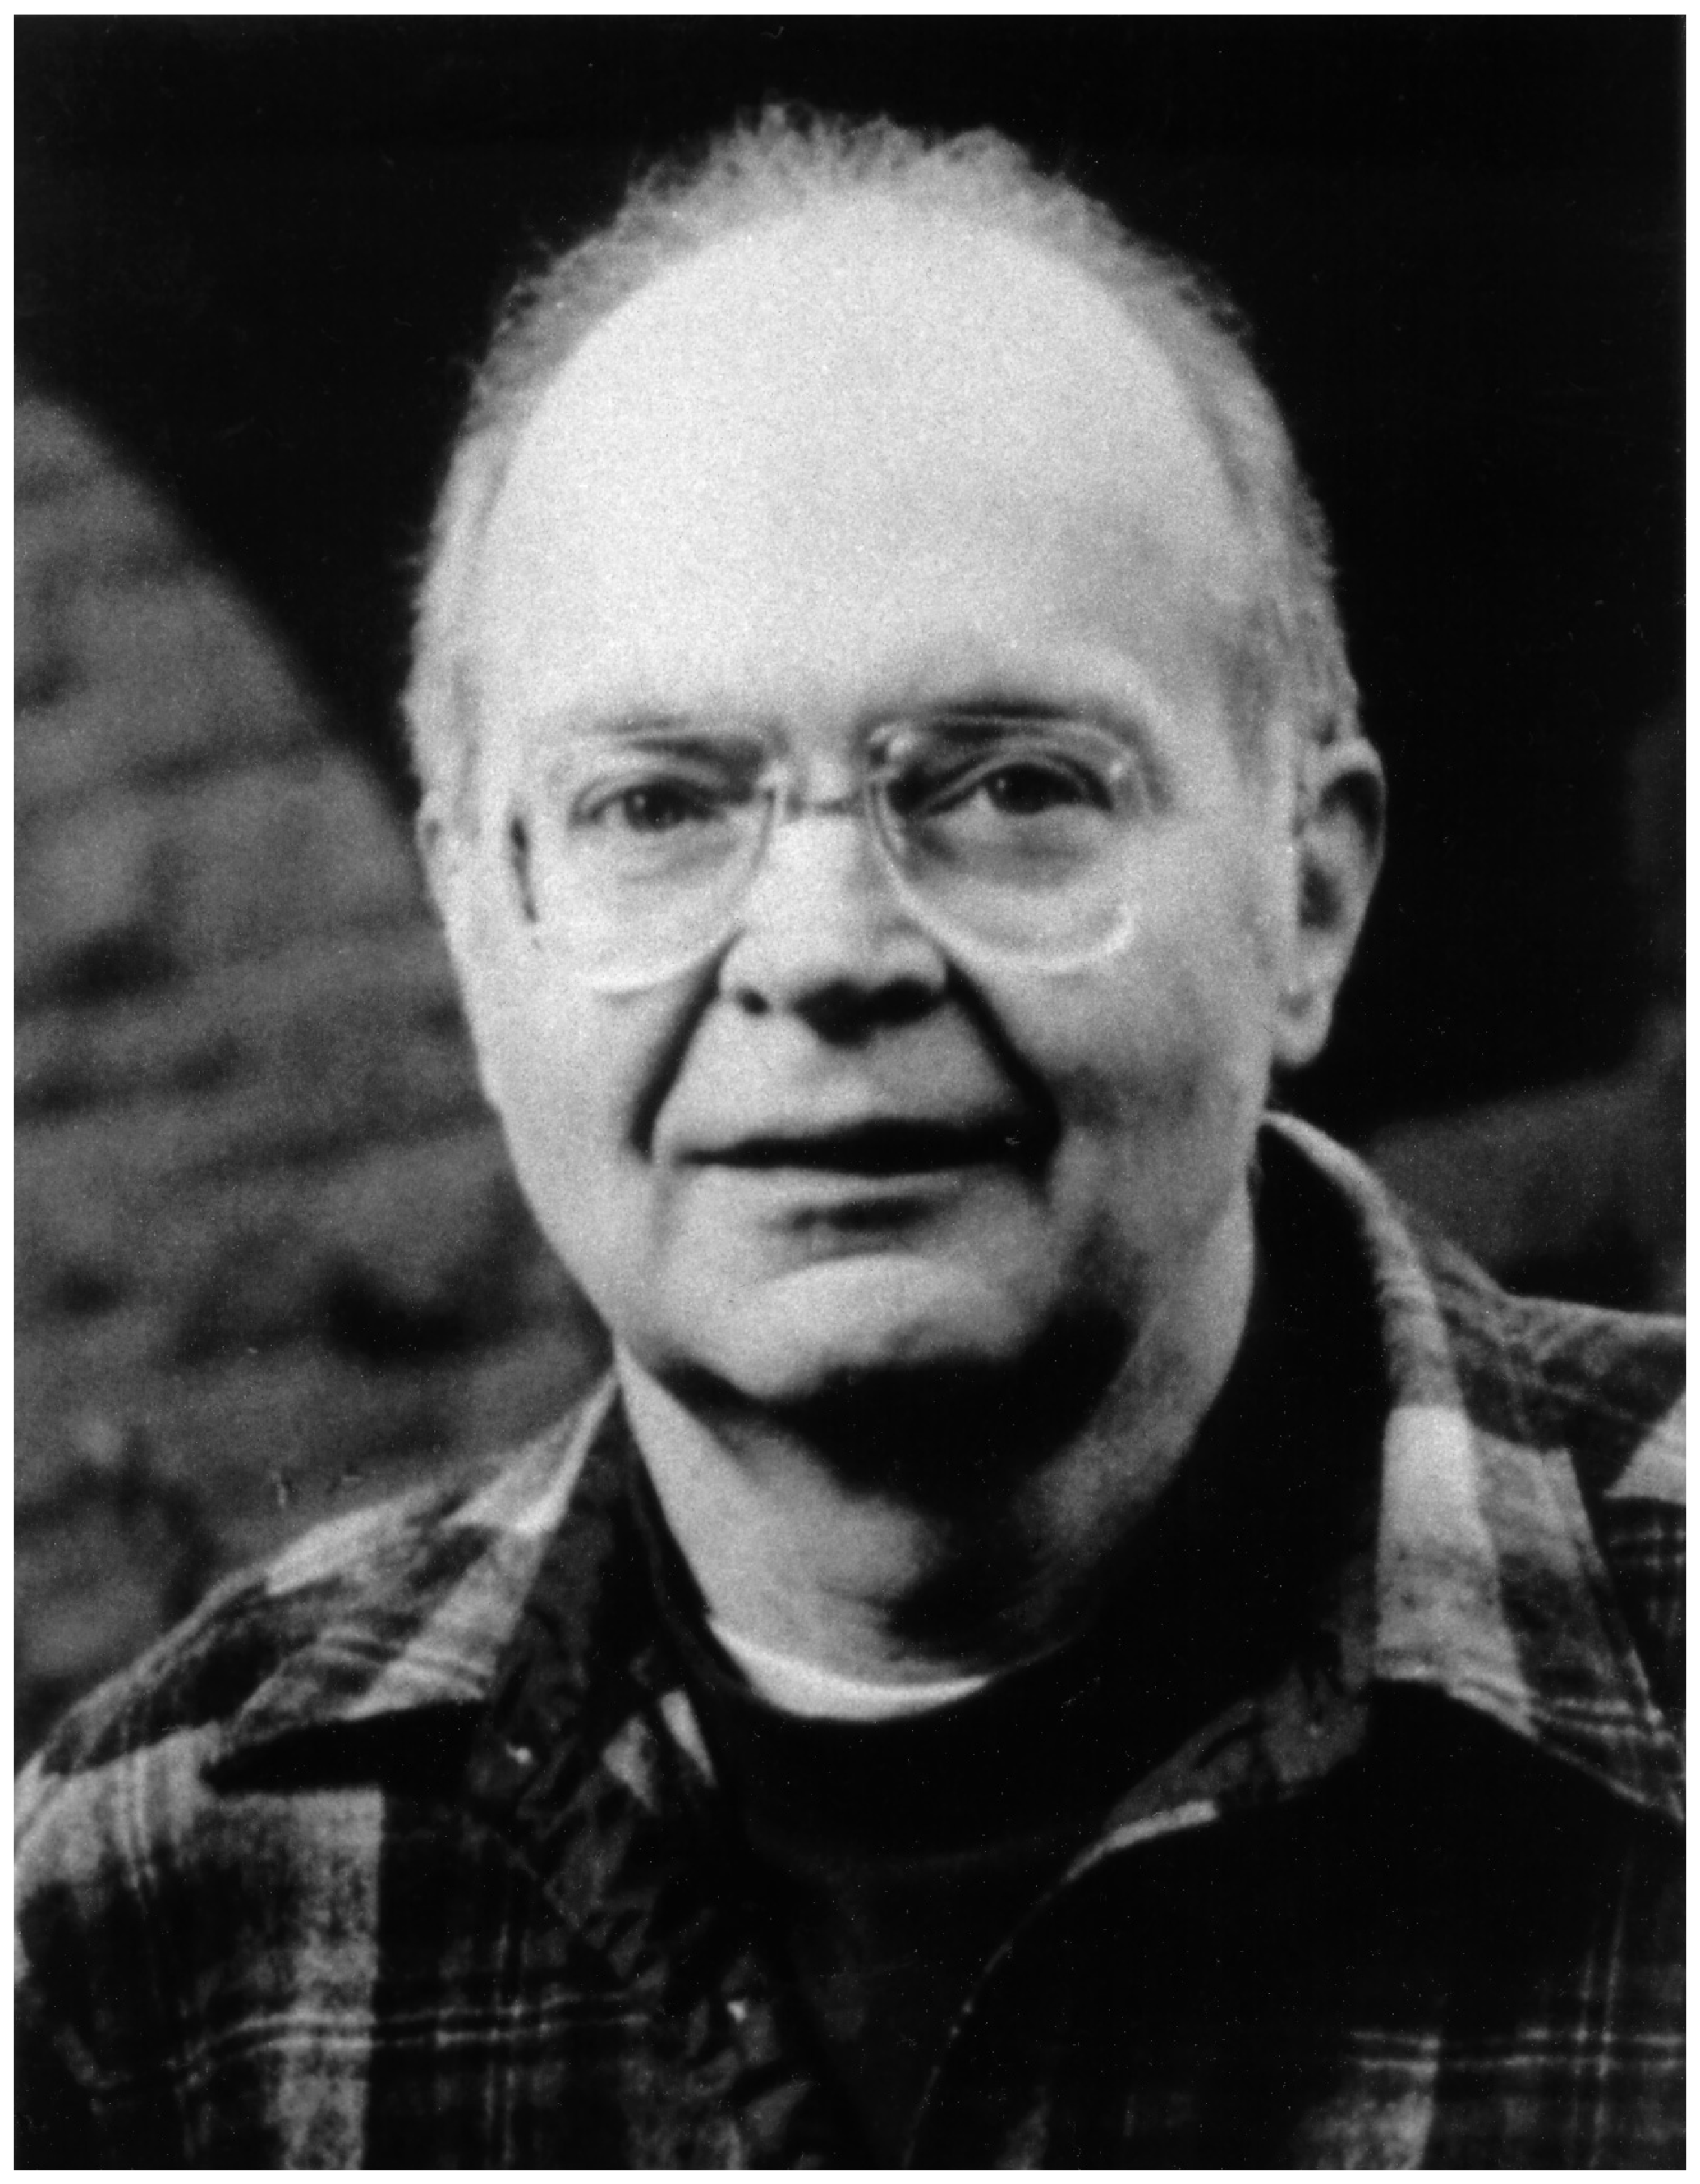
\includegraphics[height=2cm]{don-hires}}
  \caption{包含子图形的大图形}
  \label{fig:big1}
\end{figure}

培育英才万万千,建设祖国锦绣河山,华师儿女奋勇当先,珠江滚滚红绵艳~,岭南大地草木
春,改革开放阳光好,华师园里花烂漫。

艰苦奋斗众志坚,严谨治学成风范,求实创新勇开拓,为人师表代代相传,教育改革宏图展,
师范园地好摇篮,培育祖国栋梁材,神圣职责我承担。


下面这个例子显示并排$3\times2$的图片,见图\ref{fig:subfig:3x2}:
\begin{figure}[htb]
\centering
\subfloat[]{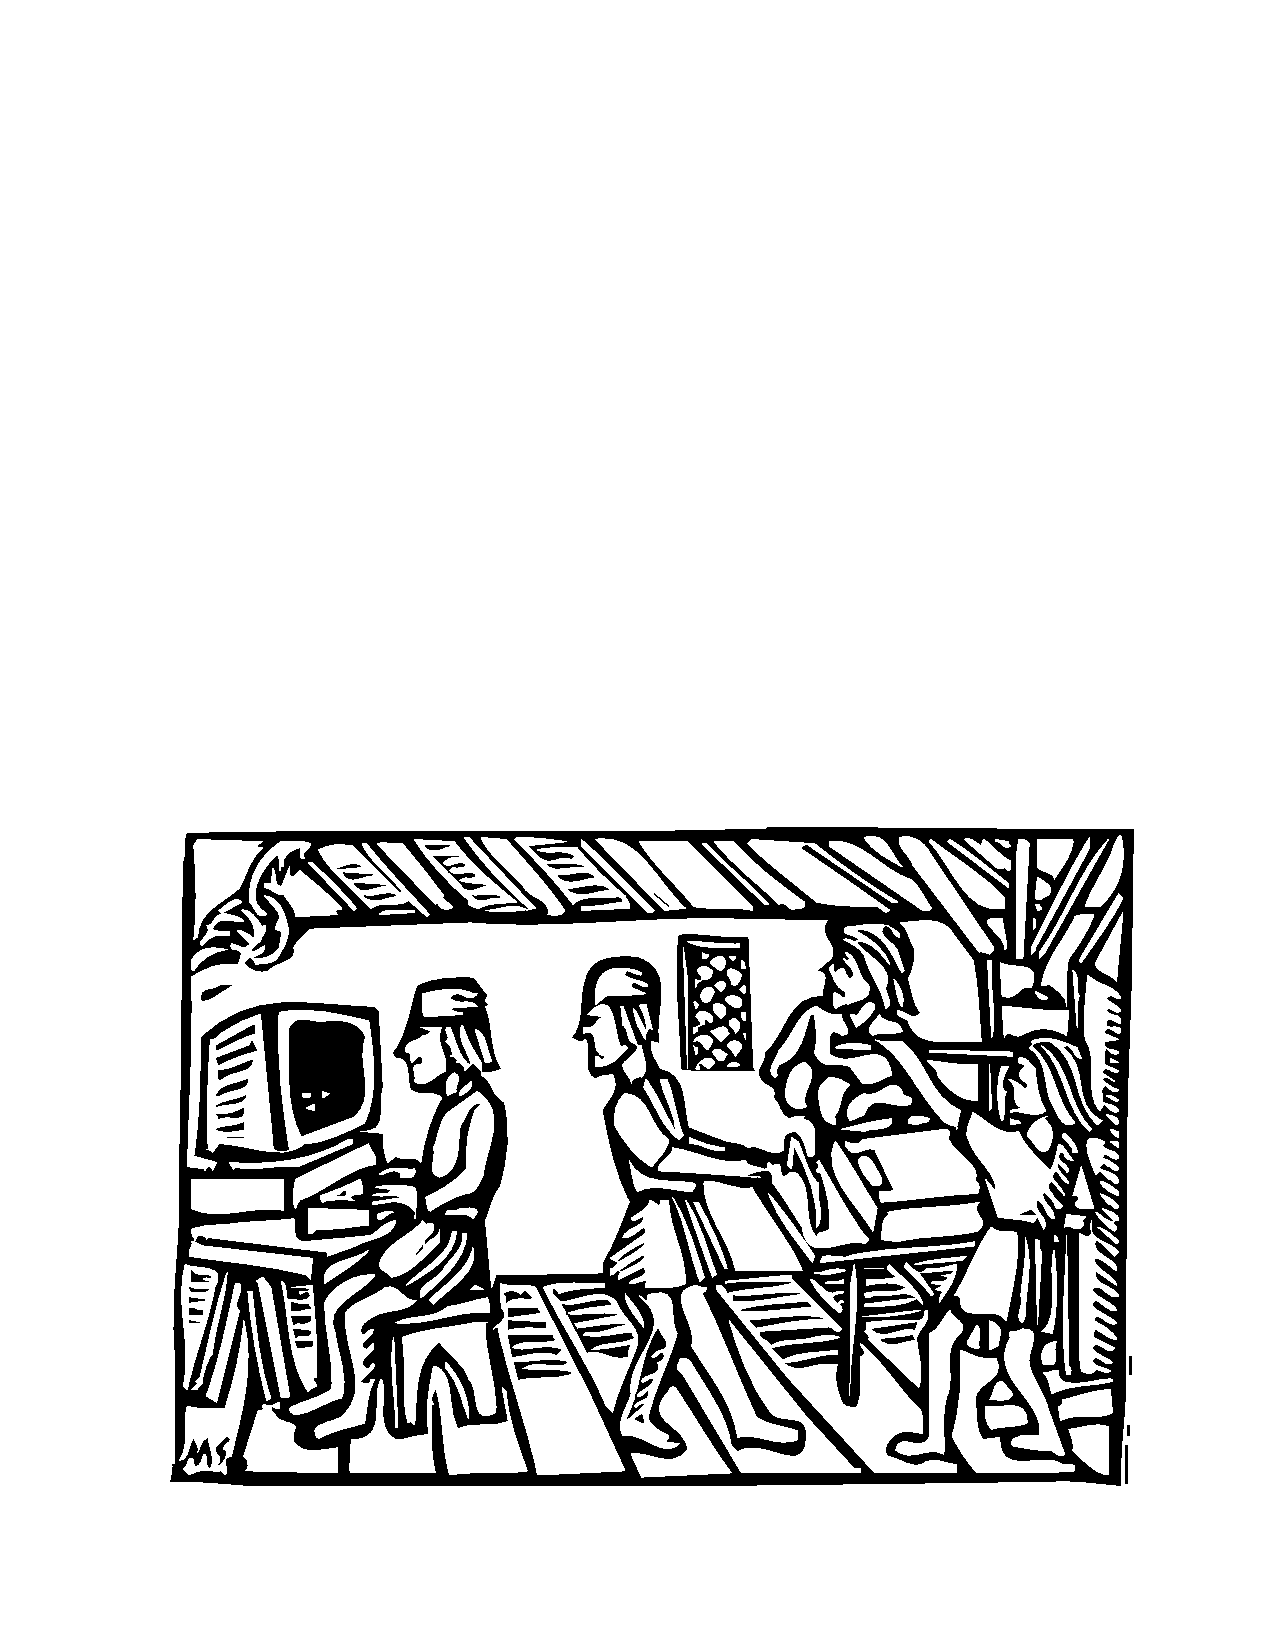
\includegraphics[width=.27\textwidth]{typography}} \qquad
\subfloat[]{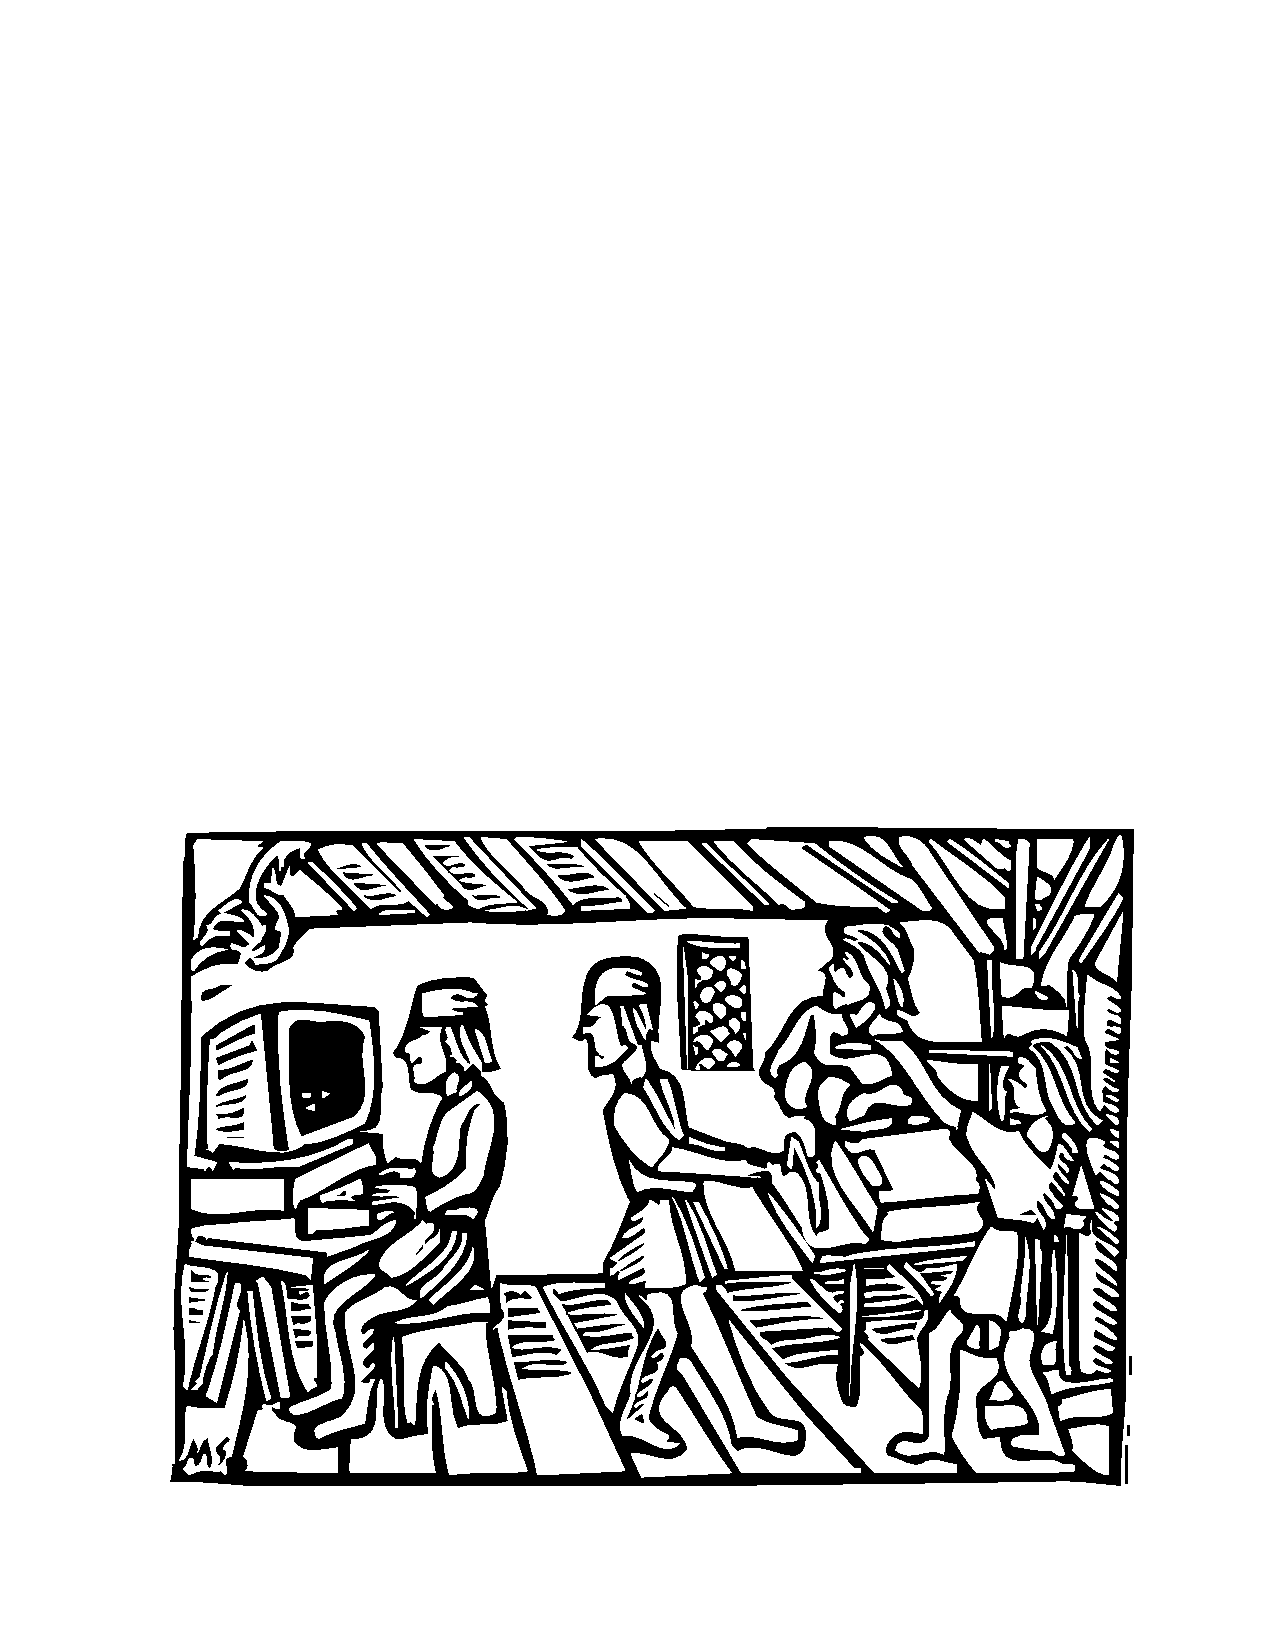
\includegraphics[width=.27\textwidth]{typography}} \qquad
\subfloat[]{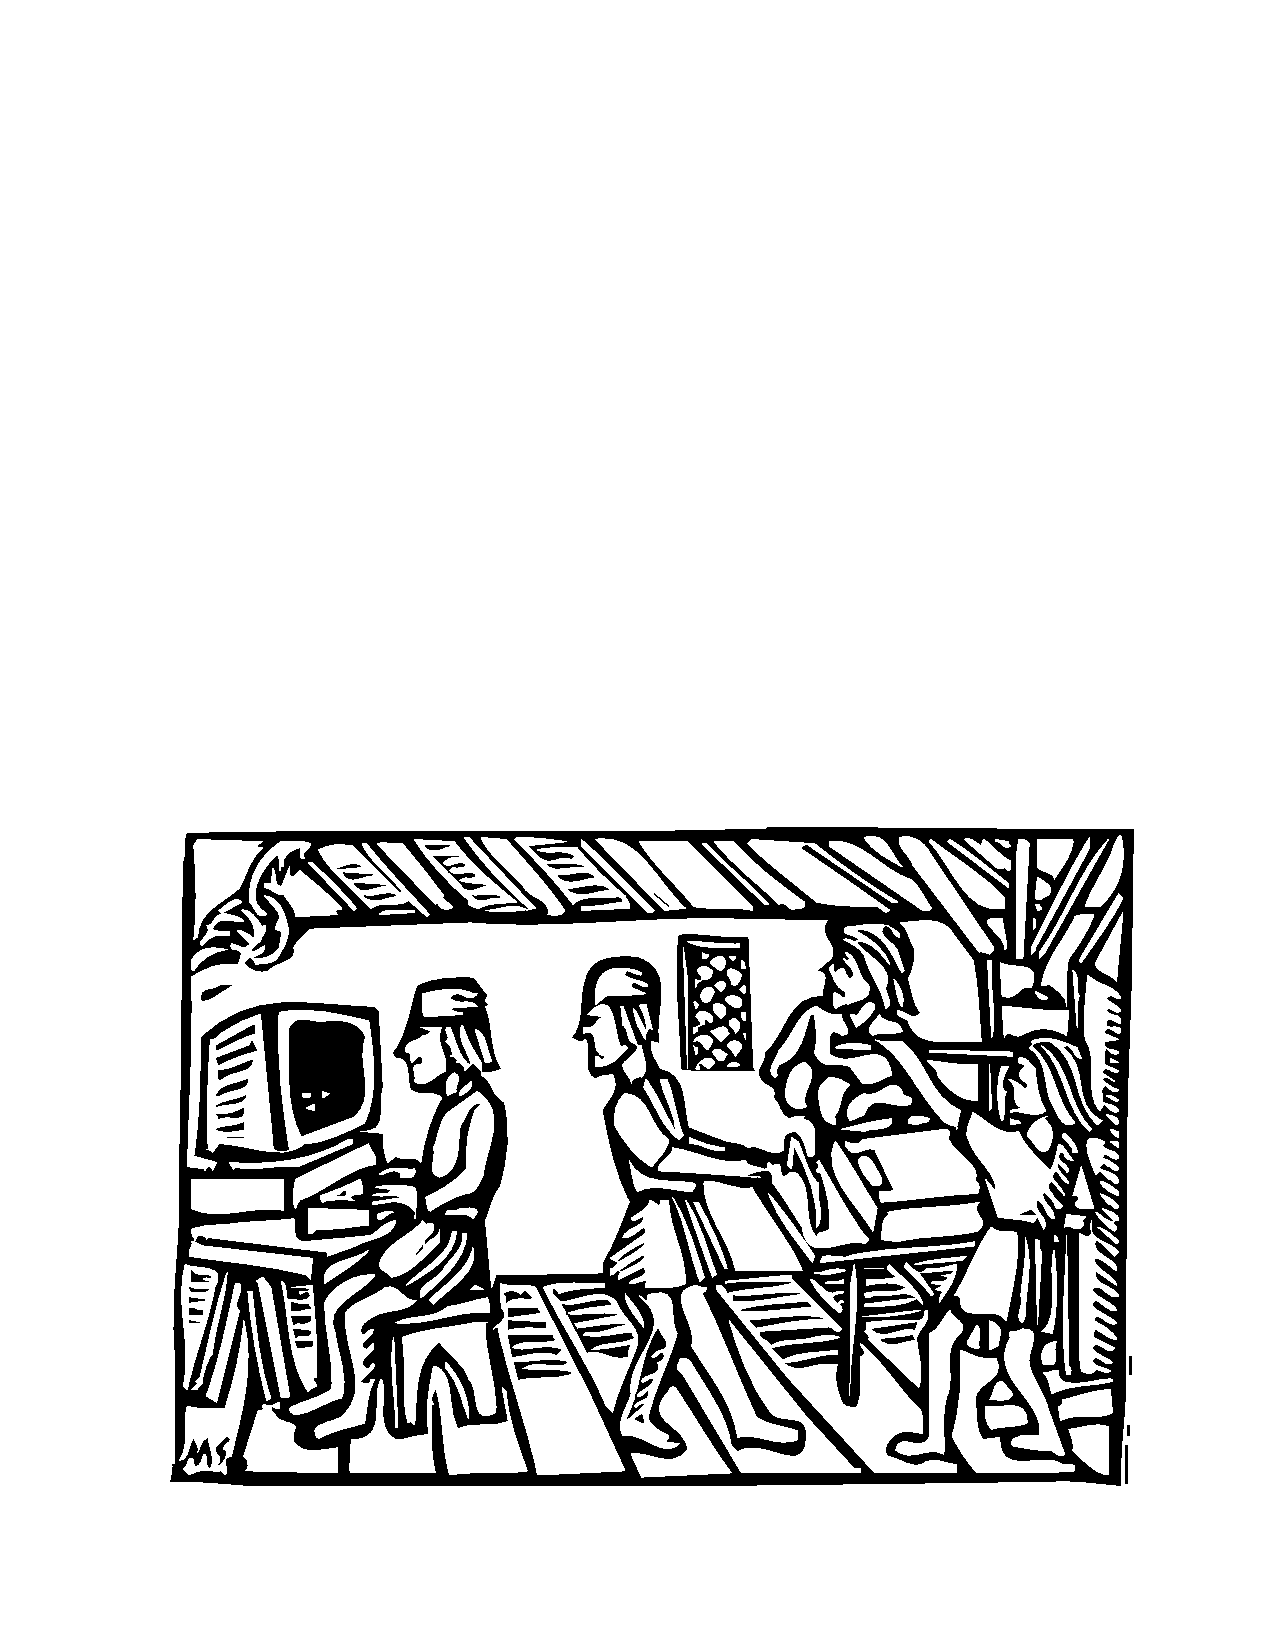
\includegraphics[width=.27\textwidth]{typography}} \qquad
\subfloat[]{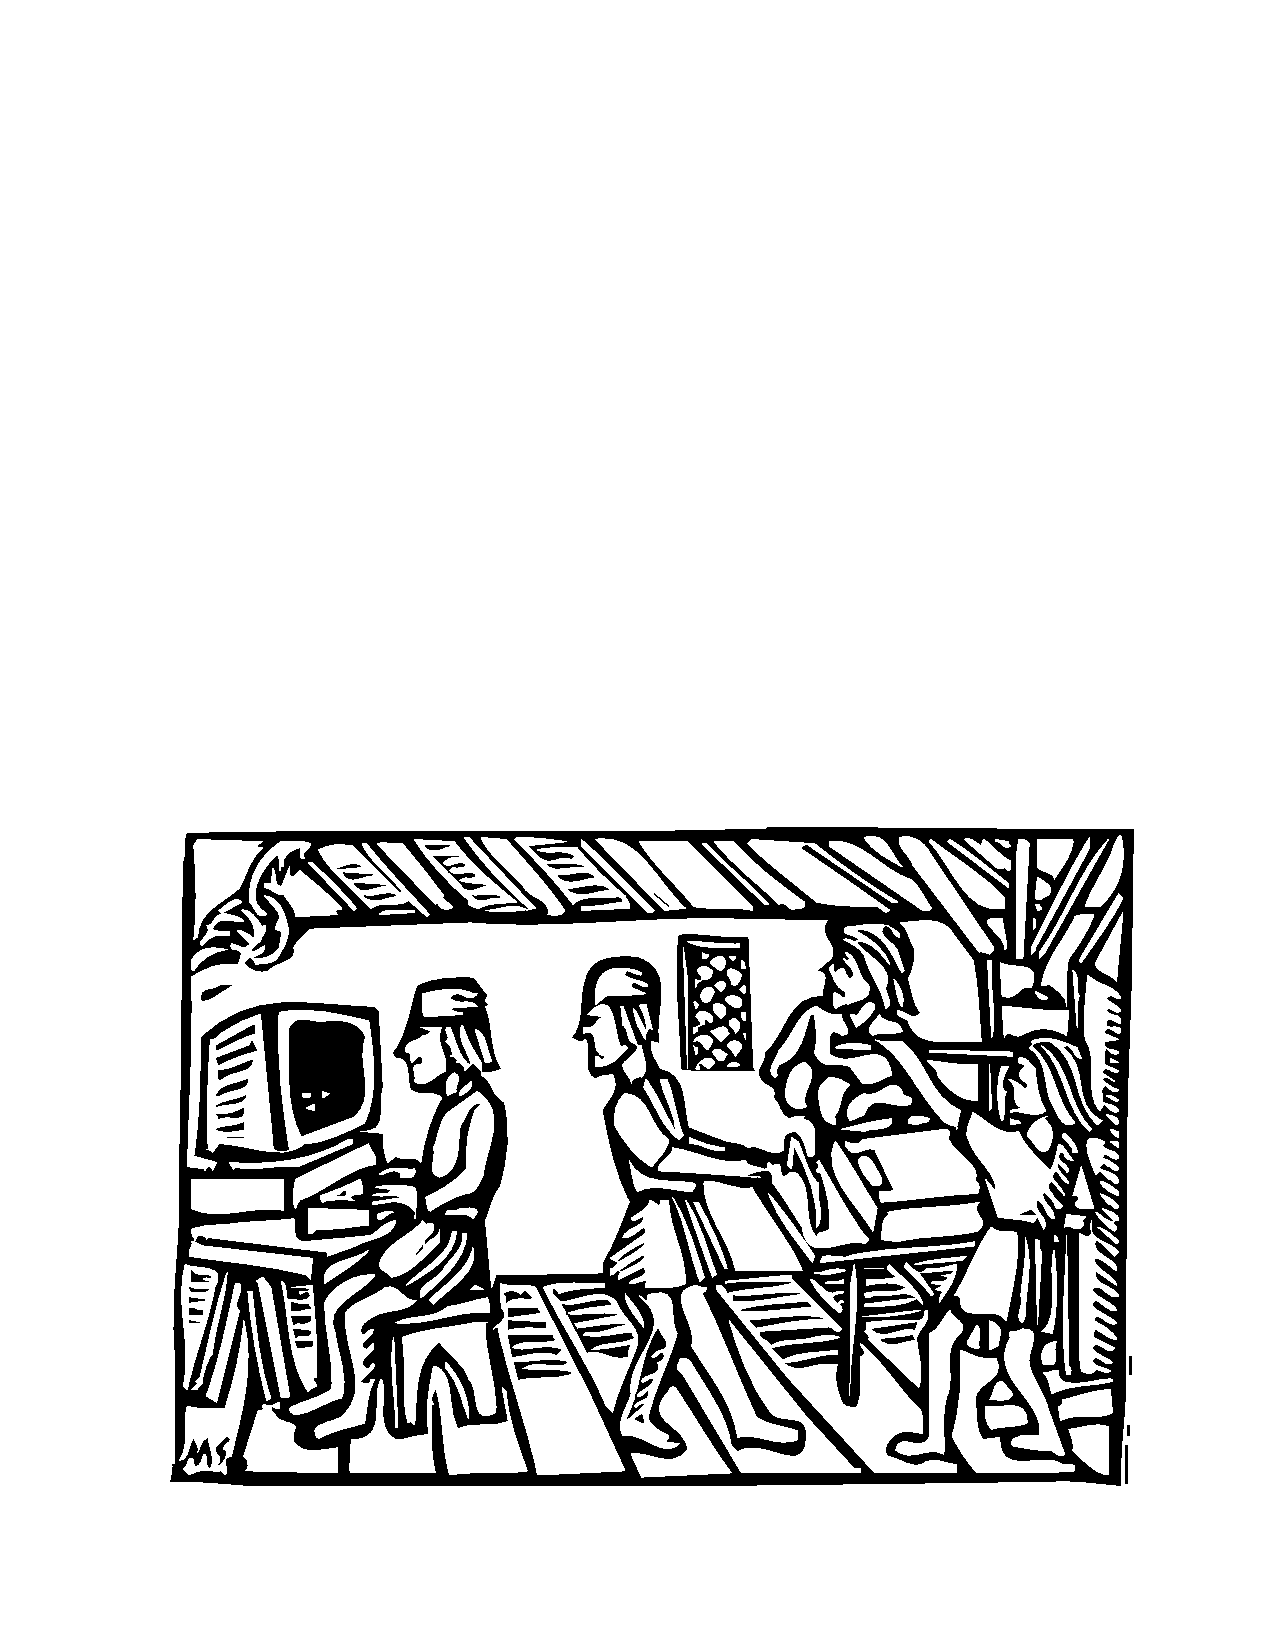
\includegraphics[width=.27\textwidth]{typography}} \qquad
\subfloat[]{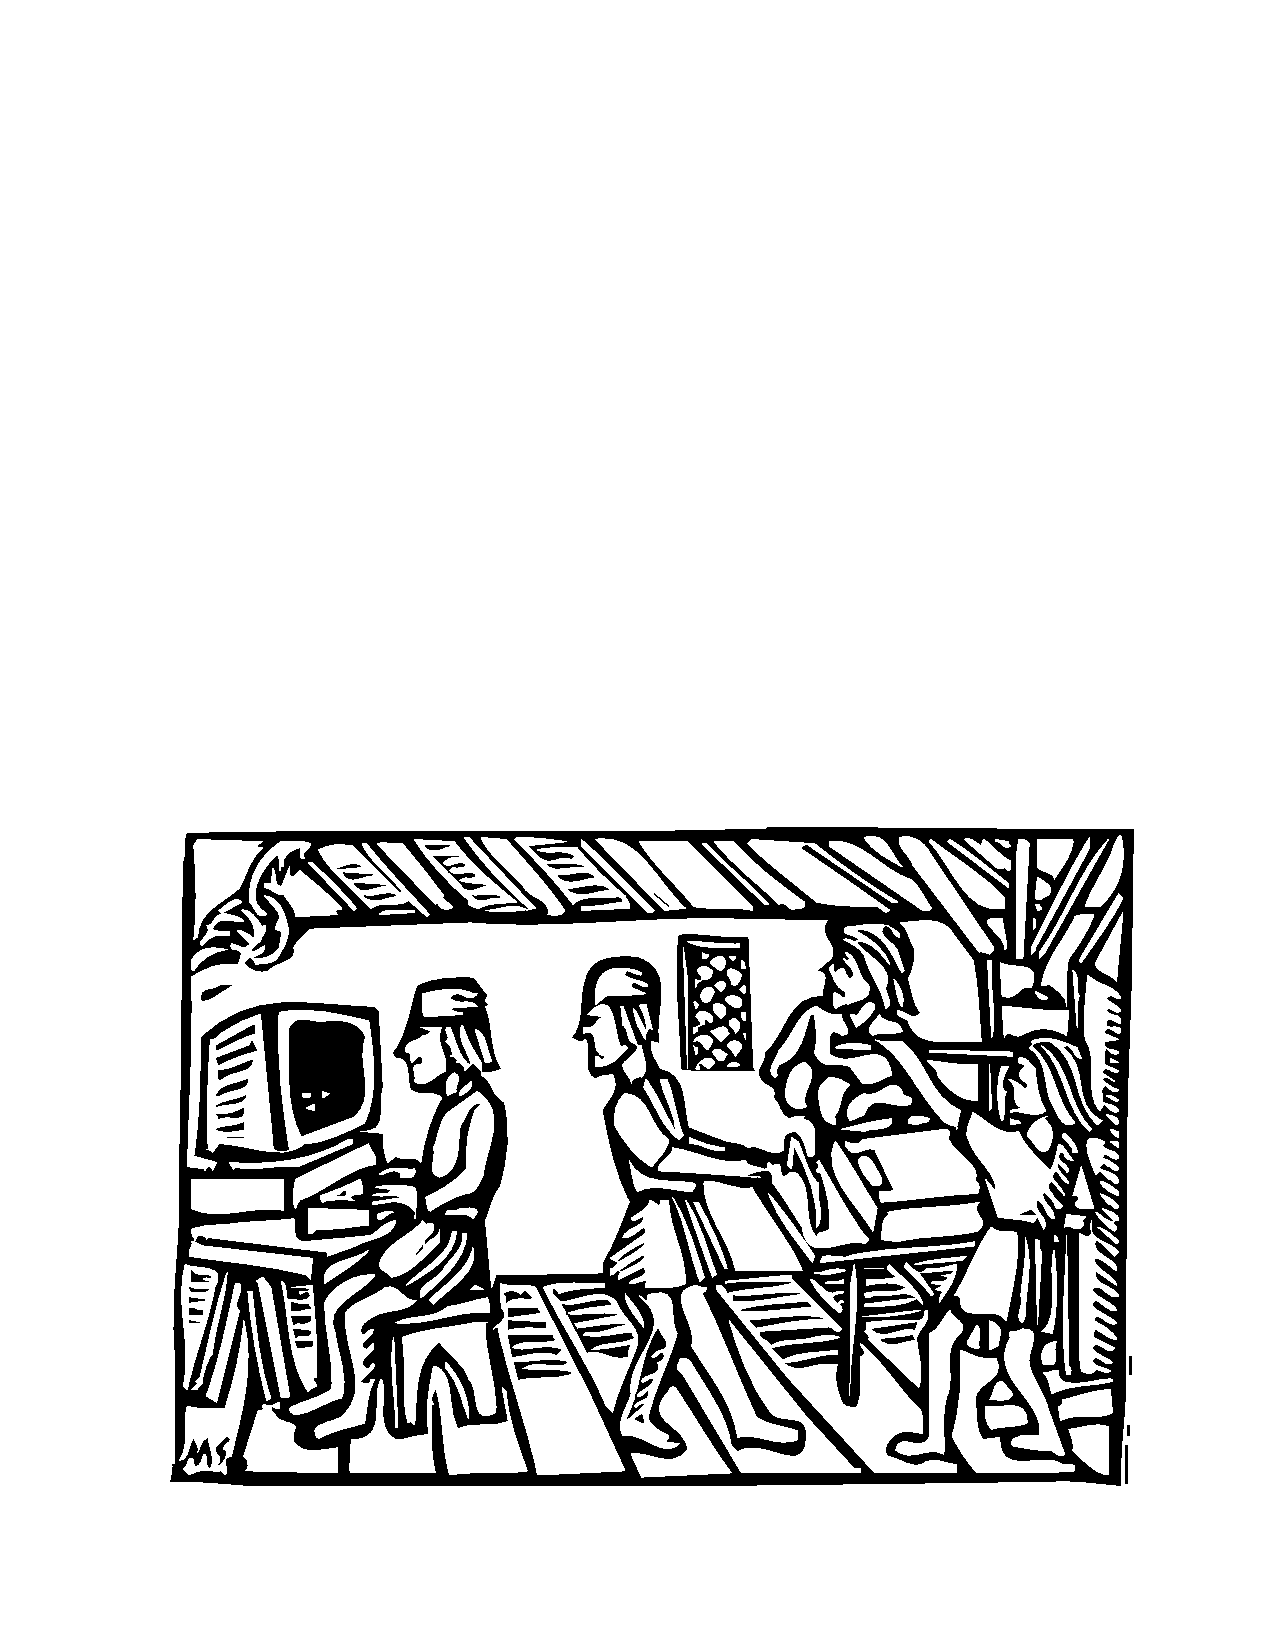
\includegraphics[width=.27\textwidth]{typography}} \qquad
\subfloat[]{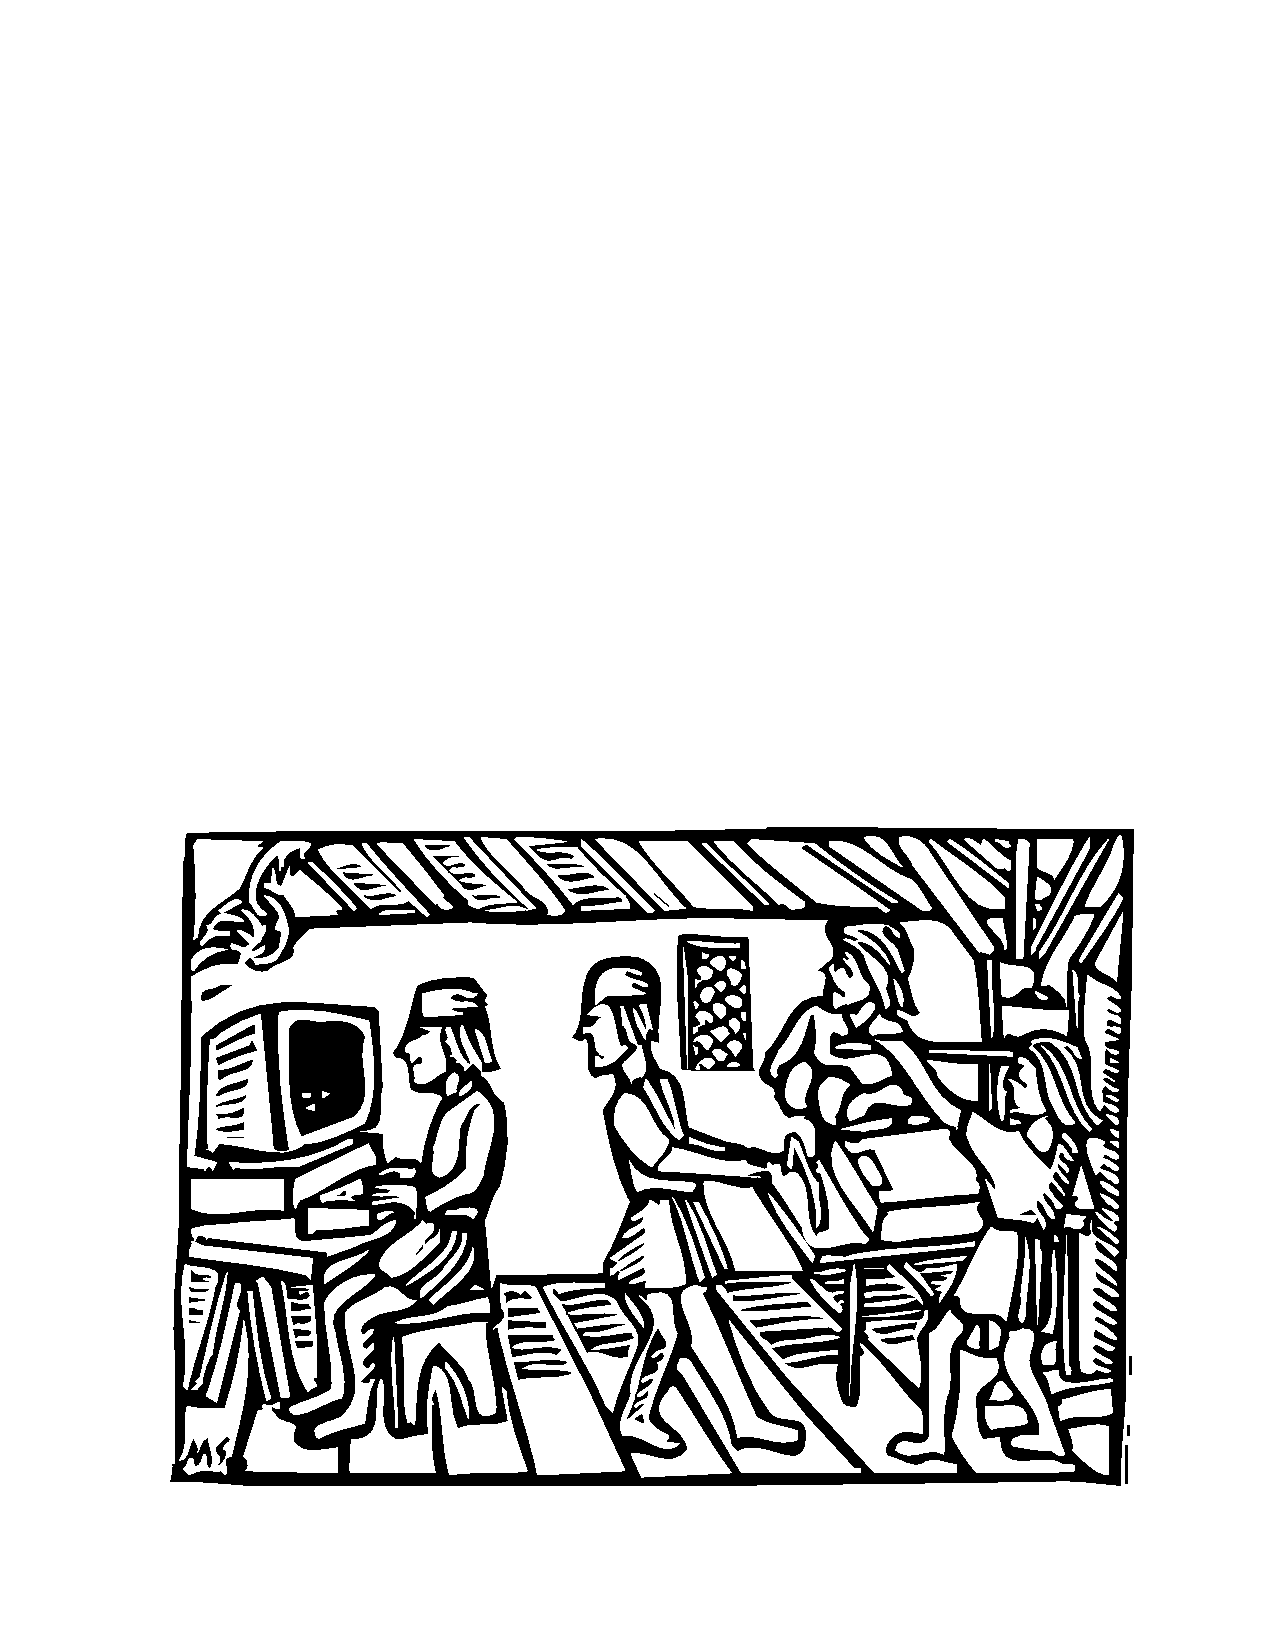
\includegraphics[width=.27\textwidth]{typography}}
\caption{并排图片}
\label{fig:subfig:3x2}
\end{figure}

要注意,\texttt{qquad}相当于\verb|\hspace{2em}|,也就是2个字符的宽度,约0.08倍页宽,
图片宽度设定为0.27倍页宽是合适的;在该环境中,尽量不要手动换行。

向前向前向前向前,华师儿女永远向前!

如果要把编号的两个图形并排,那么小页就非常有用了:
\begin{figure}[htb]
\begin{minipage}{0.48\textwidth}
  \centering
  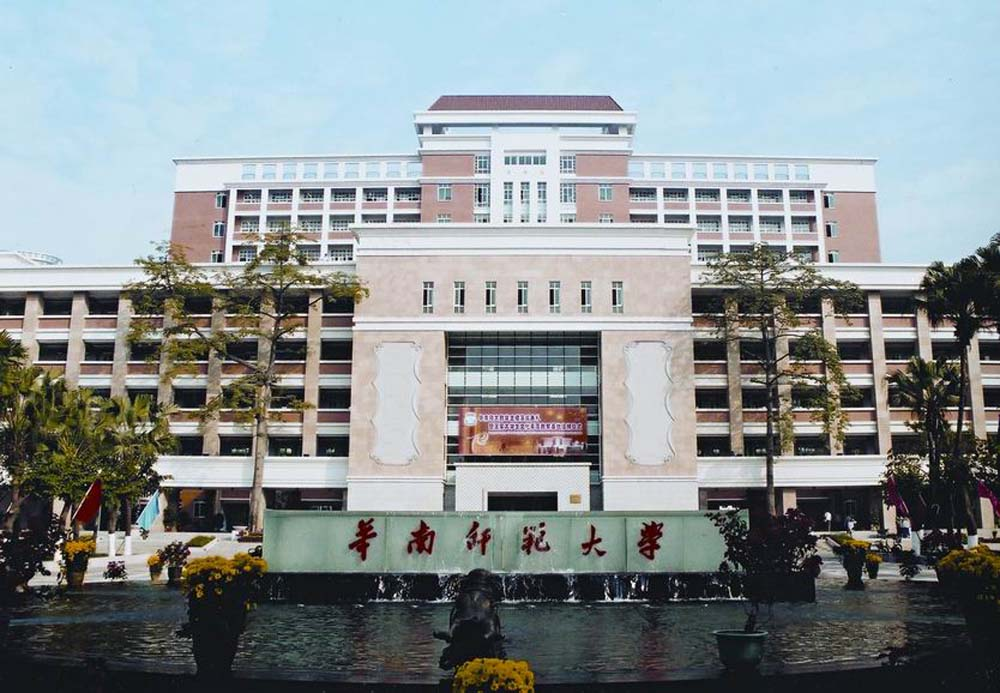
\includegraphics[height=4cm]{building.jpg}
  \caption{并排第一个图}
  \label{fig:parallel1}
\end{minipage}\hfill
\begin{minipage}{0.48\textwidth}
  \centering
  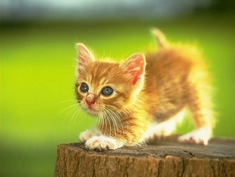
\includegraphics[height=4cm]{cat.jpg}
  \caption{并排第二个图}
  \label{fig:parallel2}
\end{minipage}
\end{figure}

\section{公式定理}
\label{sec:equation}
贝叶斯公式如式~(\ref{equ:chap1:bayes}),其中 $p(y|\mathbf{x})$ 为后验;
$p(\mathbf{x})$ 为先验;分母 $p(\mathbf{x})$ 为归一化因子。
\begin{equation}
\label{equ:chap1:bayes}
p(y|\mathbf{x}) = \frac{p(\mathbf{x},y)}{p(\mathbf{x})}=
\frac{p(\mathbf{x}|y)p(y)}{p(\mathbf{x})} 
\end{equation}

论文里面公式越多,\TeX{} 就越 happy。再看一个 \textsf{amsmath} 的例子:
\newcommand{\envert}[1]{\left\lvert#1\right\rvert} 
\begin{equation}\label{detK2}
\det\mathbf{K}(t=1,t_1,\dots,t_n)=\sum_{I\in\mathbf{n}}(-1)^{\envert{I}}
\prod_{i\in I}t_i\prod_{j\in I}(D_j+\lambda_jt_j)\det\mathbf{A}
^{(\lambda)}(\overline{I}|\overline{I})=0.
\end{equation} 

大家在写公式的时候一定要好好看 \textsf{amsmath} 的文档,并参考模板中的用法:
\begin{multline*}%\tag{[b]} % 这个出现在索引中的
\int_a^b\biggl\{\int_a^b[f(x)^2g(y)^2+f(y)^2g(x)^2]
 -2f(x)g(x)f(y)g(y)\,dx\biggr\}\,dy \\
 =\int_a^b\biggl\{g(y)^2\int_a^bf^2+f(y)^2
  \int_a^b g^2-2f(y)g(y)\int_a^b fg\biggr\}\,dy
\end{multline*}

多列公式也是比较常见的情况,比较常用的办法是用align环境实现:

\begin{equation} 
\mathbf{X} = \left(\begin{array}{ccc} 
x_{11} & x_{12} & \ldots \\ 
x_{21} & x_{22} & \ldots \\ 
\vdots & \vdots & \ddots \end{array} \right) 
\end{equation} 

\begin{equation} 
y = \left\{ \begin{array}{ll} 
a & \textrm{if $d>c$}\\ 
b+x & \textrm{in the morning}\\ 
l & \textrm{all day long} 
\end{array} \right. 
\end{equation} 

\begin{equation} 
\left(\begin{array}{c|c} 
1 & 2 \\ 
\hline 3 & 4 \end{array}\right) 
\end{equation}   

\begin{eqnarray}
f(x) & = & \cos x \\ 
f'(x) & = & -\sin x \\ 
\int_{0}^{x} f(y)\,dy & = & \sin x 
\end{eqnarray} 

{\setlength\arraycolsep{2pt} 
\begin{eqnarray} 
\sin x & = & x -\frac{x^{3}}{3!} +\frac{x^{5}}{5!}-{} \nonumber\\ 
	& & {}-\frac{x^{7}}{7!}+{}\cdots 
\end{eqnarray}} 

另外,\texttt{split}环境可能在XeCJK上不能使用,我们测试一下,看\ref{equ:split}:
\begin{equation}\label{equ:split}
\begin{split}
[z^n]C(z) &= [z^n] \biggl[\frac{e^{3/4}}{\sqrt{1-z}} +
e^{-3/4}(1-z)^{1/2} + \frac{e^{-3/4}}{4}(1-z)^{3/2}
+ O\Bigl( (1-z)^{5/2}\Bigr)\biggr] \\
&= \frac{e^{-3/4}}{\sqrt{\pi n}} - \frac{5e^{-3/4}}{8\sqrt{\pi
n^3}} + \frac{e^{-3/4}}{128 \sqrt{\pi n^5}} +
O\biggl(\frac{1}{\sqrt{\pi
n^7}}\biggr)
\end{split}
\end{equation}
\textbf{注意:} 论文模板中为了与xeCJK稳定版本兼容,调校了split命令,代价是不能在inline使用split命令。

\begin{theorem}
  \label{chapTSthm:rayleigh solution}
  假定 $X$ 的二阶矩存在:
  \begin{equation}
         O_R(\textbf{x},F)=\sqrt{\frac{\textbf{u}_1^T\textbf{A}\textbf{u}_1} {\textbf{u}_1^T\textbf{B}\textbf{u}_1}}=\sqrt{\lambda_1},
  \end{equation}
  其中 $\textbf{A}$ 等于 $(\textbf{x}-EX)(\textbf{x}-EX)^T$,\textbf{B} 表示协方差阵 $E(X-EX)(X-EX)^T$,$\lambda_1$
$\textbf{u}_1$ 是 $\lambda_1$对应的特征向量, $\omega,\ve{\omega},\omegaup,\ve{\omegaup}$.
\end{theorem}

\begin{proof}
 上述优化问题显然是一个 Rayleigh 商问题。我们有
  \begin{align}
     O_R(\textbf{x},F)=\sqrt{\frac{\textbf{u}_1^T\textbf{A}\textbf{u}_1} {\textbf{u}_1^T\textbf{B}\textbf{u}_1}}=\sqrt{\lambda_1},
 \end{align}
 其中 $\lambda_1$ 下列广义特征值问题的最大特征值:
$$
\textbf{A}\textbf{z}=\lambda\textbf{B}\textbf{z}, \textbf{z}\neq 0.
$$
 $\textbf{u}_1$ 是 $\lambda_1$对应的特征向量。结论成立。
\end{proof}

\subsection{非回路故障的推理算法}
我们知道,故障诊断的最终目的,是将故障定位到部件,而由于信号-部件依赖矩阵的存在,因此,实质性的工作是找出由故障部件发出异常信号,
不妨称为源异常信号,而如前所述,源异常信号与异常信号依赖矩阵$\mathbf{S_a}$的全零列是存在一一对应的关系的。因此,我们只要获得了$\mathbf{S_a}$的全零列的相关信息,
也就获得了源异常信号的信息,从而能进一步找到故障源。
通过以上分析,我们构造算法\ref{alg53},用于实现非回路故障诊断。

算法\ref{alg53}中,称$\beta$为源异常信号向量,该向量中与源异常信号对应的元素值为1,其它为0;
称$\gamma$为部件状态向量,该向量中非0元素对应的部件为故障部件~,0元素对应的部件为正常部件。
值得一提的是$\beta$和$\beta_a$的区别。$\beta$指出了源异常信号在所有信号中排序的位置,因此其维数与信号总数相同;
而$\beta_a$指出了源异常信号在所有异常信号中排序的位置,因此其维数与异常信号总数相同。如前所述,信号的“排序”是固定的,
这保证了算法在执行中不出现混乱。
\begin{algorithm}[htbp]
  \caption{非回路故障诊断算法}
  \label{alg53}
  \begin{algorithmic}[1]
    \REQUIRE 信号--部件依赖矩阵$\mathbf{A}$,信号依赖矩阵$\mathbf{S}$,信号状态向量$\alpha$
    \ENSURE 部件状态向量$\gamma$
    \STATE $\mathbf{P}\leftarrow\left(<\alpha>\right)$
    \STATE $\mathbf{S_{a}}\leftarrow\mathbf{P^T}\mathbf{S}\mathbf{P}$
    \FOR{$i=1$ to $S_a$的阶数$m$}
    \STATE $s_i\leftarrow s_i$的第$i$个行向量
    \ENDFOR
    \STATE $\beta_a\leftarrow\lnot \left(s_1\lor s_2\lor \cdots\lor s_m\right)^T$
    \STATE $\beta\leftarrow\mathbf{P}\beta_a$
    \STATE $\gamma\leftarrow\mathbf{A}\beta$
  \end{algorithmic}
\end{algorithm}
\subsubsection{第一类故障回路的推理算法}
第一类故障回路推理与非回路故障推理是算法基本相同,稍微不同的是$\beta_a$的计算。因为第一类故障回路中的信号全部可能是源异常信号,因此我们不必计算
$\beta_a=\lnot \left(\left[s_1\lor s_2\lor \cdots\lor s_m\right]^T\right)$,而直接取$\beta_a=\underbrace{\left[\begin{array}{cccc}1&1&\cdots&1\end{array}\right]^T}_m$,将$\beta_a$代入
算法\ref{alg53},有
\[\beta=\mathbf{P}\beta_a=\mathbf{P}\underbrace{\left[\begin{array}{cccc}1&1&\cdots&1\end{array}\right]^T}_m=\alpha\]
因此一类故障回路的推理算法变得相当简单,例如算法\ref{alg54}
\begin{algorithm}[htbp]
  \caption{第一类故障回路诊断算法}
  \label{alg54}
  \begin{algorithmic}[1]
    \REQUIRE 信号--部件依赖矩阵$\mathbf{A}$,信号状态向量$\alpha$
    \ENSURE 部件状态向量$\gamma$
    \STATE $\gamma\leftarrow\mathbf{A}\alpha$
  \end{algorithmic}
\end{algorithm}

\section{参考文献}
\label{sec:bib}
当然参考文献可以直接写 bibitem,虽然费点功夫,但是好控制,各种格式可以自己随意改
写,在\scnuthesis{}里面,建议使用JabRef编辑和管理文献,再结合\verb|bstutf8.bst|之后,
对中文的支持也很好。

本模板推荐使用 BIB\TeX,样式文件为 bstutf8.bst,基本符合学校的参考文献格式(如专利
等引用未加详细测试)。看看这个例子,关于书的\upcite{tex, companion},
还有这些\upcite{clzs},关于杂志的\upcite{ELIDRISSI94,
  MELLINGER96, SHELL02},硕士论文\upcite{zhubajie, metamori2004},博士论文
\upcite{shaheshang, FistSystem01},标准文件\upcite{IEEE-1363}~,会议论文\upcite{DPMG},%
技术报告\upcite{NPB2}。中文参考文献\upcite{cnarticle}\textsf{特别注意},需要在\verb|bibitem|中
增加\verb|language|域并设为\verb|zh|,英文此项可不填,之后由\verb|bstutf8|统一处理
(具体就是决定一些文献的显示格式,如等、etc)。
若使用\verb|JabRef|,则选择\textsf{Options}$\rightarrow$\textsf{Set Up General Fields},
在\verb|General:|后加入\verb|language|就可以了。

有时候不想要上标,那么可以这样 \cite{shaheshang},这个非常重要。

\section{代码高亮}
有些时候我们需要在论文中引入一段代码,用来衬托正文的内容,或者体现关键思路的实现。
在模板中,统一使用\texttt{listings}宏包,并且设置了基本的内容格式,并建议用户只
使用三个接口,分别控制:编程语言,行号以及边框。简洁达意即可,下面分别举例说明。

首先是设定语言,来一个C的,使用的是默认设置:
\begin{lstlisting}[language=C]
void sort(int arr[], int beg, int end)
{
  if (end > beg + 1)
  {
    int piv = arr[beg], l = beg + 1, r = end;
    while (l < r)
    {
      if (arr[l] <= piv)
        l++;
      else
        swap(&arr[l], &arr[--r]);
    }
    swap(&arr[--l], &arr[beg]);
    sort(arr, beg, l);
    sort(arr, r, end);
  }
}
\end{lstlisting}

当我们需要高亮Java代码,不需要行号,不需要边框时,可以:
\begin{lstlisting}[language=Java,numbers=none,frame=none]
// A program to display the message
// "Hello World!" on standard output

public class HelloWorld {
 
   public static void main(String[] args) {
      System.out.println("Hello World!");
   }
      
}   // end of class HelloWorld
\end{lstlisting}

细心的用户可能发现,行号被放在了正文框之外,事实上这样是比较美观的,如果有些用户希望在正文框架之内布置所有内容,
可以:
\begin{lstlisting}[language=perl,xleftmargin=2em,framexleftmargin=1.5em]
#!/usr/bin/perl
print "Hello, world!\n";
\end{lstlisting}

好了,就这么多,\texttt{listings}宏包的功能很强大也很复杂,如果需要自己定制,可以
查看其手册,耐心阅读总会找到答案。\textbf{注意:} 当前中文注释的处理还不是很完善,
对于注释请妥善处理。在本模板中,推荐算法环境或者去掉中文的listings代码环境。如果
需要包含中文注释,不要求代码高亮~,就用\texttt{code}环境,这个环境是Verbatim的定制
版,调用的fancyvbr宏包,用户可在myscnu.sty中修改。

\begin{code}
public class HelloWorld {
   public static void main(String[] args) {
      System.out.println("Hello World!");
   }
}   // 世界,你好!
\end{code}

\section{中文习惯}
\label{sec:chinese}

对于itermize过大的行间距,用户可以使用compactitem环境来替代,但是模板中不进行默认替代,
因为只有用户真正发现列表不好看才会找到这里。

对于中文双引号,可以直接使用全角的\verb|“|和\verb|”|。但是英文则不行!英文的引
号用法请自行Google,或者阅读我的
\href{https://dl.dropbox.com/u/49734213/LaTeX%E6%9C%AD%E8%AE%B0.pdf}{\LaTeX{}}札
记。

中文破折号为一个两个字宽垂直居中的直线,输入法直接得到的破折号没有垂直居中(——),
这看起来不舒服。所以模板中定义了一个破折号的命令 \verb|\pozhehao|,请看:

艰苦奋斗、严谨治学、求实创新、为人师表\hfill \pozhehao{}华南师范大学校训
\chapter{结论}
\label{chap:conclusion}

如来道:“圣僧,汝前世原是我之二徒,名唤金蝉子。因为汝不听说法,轻慢
我之大教,故贬汝之真灵,转生东土。今喜皈依,秉我迦持,又乘吾教,取去真经,
甚有功果,加升大职正果,汝为旃檀功德佛。孙悟空,汝因大闹天宫,吾以甚深法
力,压在五行山下,幸天灾满足,归于释教;且喜汝隐恶扬善,在途中炼魔降怪有
功,全终全始,加升大职正果,汝为斗战胜佛。猪悟能,汝本天河水神,天蓬元帅。
为汝蟠桃会上酗酒戏了仙娥,贬汝下界投胎,身如畜类。幸汝记爱人身,在福陵山
云栈洞造孽,喜归大教,入吾沙门,保圣僧在路,却又有顽心,色情未泯。因汝挑
担有功,加升汝职正果,做净坛使者。”八戒口中嚷道:“他们都成佛,如何把我
做个净坛使者?”如来道:“因汝口壮身慵,食肠宽大。盖天下四大部洲,瞻仰吾
教者甚多,凡诸佛事,教汝净坛,乃是个有受用的品级。如何不好——沙悟净,汝
本是卷帘大将,先因蟠桃会上打碎玻璃盏,贬汝下界,汝落于流沙河,伤生吃人造
孽,幸皈吾教,诚敬迦持,保护圣僧,登山牵马有功,加升大职正果,为金身罗汉。”
又叫那白马:“汝本是西洋大海广晋龙王之子。因汝违逆父命,犯了不孝之罪,幸
得皈身皈法,皈我沙门,每日家亏你驮负圣僧来西,又亏你驮负圣经去东,亦有功
者,加升汝职正果,为八部天龙。”

因此:

\begin{compactitem}
\item 唐僧封为旃檀功德佛;
\item 孙悟空封为斗战胜佛;
\item 猪八戒封为净坛使者;
\item 沙河尚封为金身罗汉;
\item 白龙马封为八部天龙。
\item 华师是个好学校。
\end{compactitem}




%</thesis>
%    \end{macrocode}
%<thesis>% 参考文献
%    \begin{macrocode}
%<*thesis>
\cleardoublepage
\renewcommand{\chapterlabel}{\bibname} % 设置参考文献的页眉
\bibliographystyle{bstutf8}
\bibliography{ref/refs}

%</thesis>
%    \end{macrocode}
% \subsection{后置部分}
%
% 后置部分包括附录、致谢、作者攻读学位期间发表的学术论文目录、学位论
% 文原创性声明、学位论文使用授权声明。
% 
% \changes{v0.5.7}{2013/04/28}{将多个附录分离成多个文件}
%<thesis>% 附录
%    \begin{macrocode}
%<*thesis>
\appendix
\backmatter
%%% Local Variables: 
%%% mode: latex
%%% TeX-master: "../main"
%%% End: 

\chapter{外文资料原文}
\label{cha:engorg}
\section[First Principles]{first principles}

\subsection{Typography exists to honor content.}

Like oratory, music, dance, calligraphy -- like anything that lends its grace to language -- typography is an art that can be deliberately misused. It is a craft by which the meanings of a text (or its absence of meaning) can be clarified, honored and shared, or knowingly disguised.

In a world rife with unsolicited messages, typography must often draw attention to itself before it will be read. Yet in order to be read, it must relinquish the attention it has drawn. Typography with anything to say therefore aspires to a kind of statuesque transparency. Its other traditional role is durability: not immunity to change, but a clear superiority to fashion. Typography at its best is a visual form of language linking timelessness and time.

One of the principles of durable typography is always legibility; another is something more than legibility: some earned or unearned interest that gives its living energy to the page. It takes various forms and goes by various names, including serenity, liveliness, grace and joy.

These principles apply, in different ways, to the typography of business cards, instruction sheets and postage stamps, as well as to editions of religious scriptures, literary classics and other books that aspire to join their ranks. Within limits, the same principles apply even to stock market reports, airline schedules, milk cartons, classified ads. But laughter, grace and joy, like legibility itself, all feed on meaning, which the writer, the words and the subject, not the typographer, must generally provide.

In 1770, a bill was introduced in the English Parliament with the following provisions:
\begin{quote}$\ldots$ all women of whatever age, rank, profession, or degree, whether virgins, maids, or widows, that shall $\ldots$ impose upon, seduce, and betray into matrimony, any of His Majesty's subjects, by the scents, paints, cosmetic washes, artificial teeth, false hair, Spanish wool, iron stays, hoops, high heeled shoes {\rm [}or{\rm ]} bolstered hips shall incur the pen\-alty of the law in force against witchcraft $\ldots$ and $\ldots$ the marriage, upon conviction, shall stand null and void.
\end{quote}
The function of typography, as I understand it, is neither to further the power of witches nor to bolster the defenses of those, like this unfortunate parliamentarian, who live in terror of being tempted and deceived. The satisfactions of the craft come from elucidating, and perhaps even ennobling, the text, not from deluding the unwary reader by applying scents, paints and iron stays to empty prose. But humble texts, such as classified ads or the telephone directory, may profit as much as anything else from a good typographical bath and a change of clothes. And many a book, like many a warrior or dancer or priest of either sex, may look well with some paint on its face, or indeed with a bone in its nose.

\subsection{Letters have a life and dignity of their own.}

Letterforms that honor and elucidate what humans see and say deserve to be honored in their turn. Well-chosen words deserve well-chosen letters; these in their turn deserve to be set with affection, intelligence, knowledge and skill. Typography is a link, and it ought, as a matter of honor, courtesy and pure delight, to be as strong as the others in the chain.

Writing begins with the making of footprints, the leaving of sighs. Like speaking, it is a perfectly natural act which humans have carried to complex extremes. The typographer's task has always been to add a somewhat unnatural edge, a protective shell of artificial order, to the power of the writing hand. The tools have altered over the centuries, and the exact degree of unnaturalness desired has varied from place to place and time to time, but the character of the essential transformation between manuscript and type has scarcely changed.

The original purpose of type was simply copying. The job of the typographer was to imitate the scribal hand in a form that permitted exact and fast replication. Dozens, then hundreds, then thousands of copies were printed in less time than a scribe would need to finish one. This excuse for setting texts in type has disappeared. In the age of photolithography, digital scanning and offset printing, it is as easy to print directly from handwritten copy as from text that is typographically composed. Yet the typographer's task has little changed. It is still to give the illusion of superhuman speed and stamina -- and of superhuman patience and precision~-- to the writing hand.

Typography is just that: idealized writing. Writers themselves now rarely have the calligraphic skill of earlier scribes, but they evoke countless versions of ideal script by their varying voices and literary styles. To these blind and often invisible visions, the typographer must respond in visible terms.


\chapter{其它附录}
其它附录的内容可以放到这里,当然如果你愿意,可
以把这部分也放到独立的文件中,然后将其 \verb|\input| 到主文件中。

%</thesis>
%    \end{macrocode}
%<thesis>% 致谢
%    \begin{macrocode}
%<*thesis>
\cleardoublepage
\renewcommand{\chapterlabel}{\ackname} % 设置参考文献的页眉

%%% Local Variables:
%%% mode: latex
%%% TeX-master: "../main"
%%% End:

\begin{ack}

  首先要感谢党,感谢国家!
  
  这份模板的制作首先得到了我的导师计算机学院李兴民教授,以及计算机学院陈寅副教授的
  热心支持,衷心感谢他们的教诲和指导意见!

  除此之外,还要感谢计算机学院的卓雄辉书记、雷蕾副书记、汤庸院长、单志龙副院长、王
  立斌副教授等,感谢他们对我的鼓励和帮助。

  在做这个模板的时候也获得了其他高校的\TeX{}er们的帮助,尤其是国防科大
  的\nudtpaper{}和清华大学的\thuthesis{},如果没有这些前辈们的工作,这份模板也不
  可能这么快出来和大家见面。另外,感谢戴高远同学为这个模板提供了很多宝贵的素材和
  建议,感谢莫城为同学帮忙维护这份模板,感谢周晓倩同学参与模板的测试工作。

  感谢以上所有人的努力付出,希望\scnuthesis{}能够在未来的日子里成
  为\textit{SCNUer}们的毕业论文好帮手,帮助大家完成格式规范、排版精美的论文!

\end{ack}


%</thesis>
%    \end{macrocode}
%<thesis>% 作者攻读学位期间发表的学术论文目录
%    \begin{macrocode}
%<*thesis>
\cleardoublepage
\renewcommand{\chapterlabel}{\resumename} % 设置作者个人成果的页眉
\begin{resume}

  \section*{发表的学术论文} % 发表的和录用的合在一起

  \begin{enumerate}[{[}1{]}]
  \addtolength{\itemsep}{-.36\baselineskip}%缩小条目之间的间距,下面类似
  \item Yang Y, Ren T L, Zhang L T, et al. Miniature microphone with silicon-
    based ferroelectric thin films. Integrated Ferroelectrics, 2003,
    52:229-235. (SCI 收录, 检索号:758FZ.)
  \item 杨轶, 张宁欣, 任天令, 等. 硅基铁电微声学器件中薄膜残余应力的研究. 中国机
    械工程, 2005, 16(14):1289-1291. (EI 收录, 检索号:0534931 2907.)
  \item 杨轶, 张宁欣, 任天令, 等. 集成铁电器件中的关键工艺研究. 仪器仪表学报,
    2003, 24(S4):192-193. (EI 源刊.)
  \item Yang Y, Ren T L, Zhu Y P, et al. PMUTs for handwriting recognition. In
    press. (已被 Integrated Ferroelectrics 录用. SCI 源刊.)
  \item Wu X M, Yang Y, Cai J, et al. Measurements of ferroelectric MEMS
    microphones. Integrated Ferroelectrics, 2005, 69:417-429. (SCI 收录, 检索号
    :896KM.)
  \item 贾泽, 杨轶, 陈兢, 等. 用于压电和电容微麦克风的体硅腐蚀相关研究. 压电与声
    光, 2006, 28(1):117-119. (EI 收录, 检索号:06129773469.)
  \item 伍晓明, 杨轶, 张宁欣, 等. 基于MEMS技术的集成铁电硅微麦克风. 中国集成电路, 
    2003, 53:59-61.
  \end{enumerate}

  \section*{研究成果} % 有就写,没有就删除
  \begin{enumerate}[{[}1{]}]
  \addtolength{\itemsep}{-.36\baselineskip}%
  \item 任天令, 杨轶, 朱一平, 等. 硅基铁电微声学传感器畴极化区域控制和电极连接的
    方法: 中国, CN1602118A. (中国专利公开号.)
  \item Ren T L, Yang Y, Zhu Y P, et al. Piezoelectric micro acoustic sensor
    based on ferroelectric materials: USA, No.11/215, 102. (美国发明专利申请号.)
  \end{enumerate}
\end{resume}


\end{document}
%</thesis>
%    \end{macrocode}
%
% \textcolor{blue}{Happy \TeX{}ing! 欢迎提各式各样的意见!}
%
% \newpage\relax%
% \StopEventually{\PrintChanges}
% \clearpage
%
% \section{实现细节}
% 我们首先介绍文档模板的基本信息以及宏包和配置,
% 然后依照华南师范大学论文模板的书写规范一节一节的介绍实现步骤。
%
%
% \subsection{基本信息}
%    \begin{macrocode}
%<cls>\NeedsTeXFormat{LaTeX2e}[1999/12/01]
%<cls>\ProvidesClass{scnuthesis}
%<cfg>\ProvidesFile{scnuthesis.cfg}
%<cls|cfg>
%    \end{macrocode}
%
% \subsection{宏包配置}
%
% 当前的宏包选项在之前已经介绍了,下面是实现步骤,就是几个\verb|if|。
%    \begin{macrocode}
%<*cls>
\newif\ifismaster\ismastertrue
\newif\ifisttf\isttftrue
\DeclareOption{master}{\ismastertrue}
\DeclareOption{doctor}{\ismasterfalse}
\newif\ifisanon\isanonfalse
\DeclareOption{anon}{\isanontrue}
\newif\ifistwoside\istwosidefalse
\DeclareOption{twoside}{\istwosidetrue}
\DeclareOption{ttf}{\isttftrue}
\DeclareOption{otf}{\isttffalse}
\newif\ifisvista\isvistafalse
\DeclareOption{vista}{\isvistatrue}
\newif\ifischapter\ischapterfalse
\DeclareOption{chapterhead}{\ischaptertrue}
\DeclareOption*{\PackageWarning{scnuthesis}{Unknown Option '\CurrentOption'}}
\ProcessOptions\relax
%</cls>
%    \end{macrocode}
%
% 首先调用在文档类书写中需要的过程控制语句,在计算一些\verb|length|时要用到
%    \begin{macrocode}
%<*cls>
\RequirePackage{ifthen,calc}
%</cls>
%    \end{macrocode}
%
% 接着我们导入文本类,该模板基于标准的书籍模板book,其默认格式为单面打印。
% 博士论文如需双面打印,必须指定\verb|twoside|选项。双开的含义是章节总是
% 起在右手边,左手空白页为完全的空白页,不包含页眉页脚。
%
%    \begin{macrocode}
%<*cls>
\ifistwoside
  \LoadClass[a4paper,12pt,openright,twoside]{book}
\else
  \LoadClass[a4paper,12pt,openany]{book}
  \fi
%</cls>  
%    \end{macrocode}
%
% 我们直接用\textsf{geometry}宏包进行页面边距的设定,调用titlesec设定标题以及页眉页脚,
% 用\textsf{titletoc}设定目录格式。需要改动的可以参考这三个宏包的说明文档。
%
%    \begin{macrocode}
%<*cls>
\RequirePackage[includeheadfoot]{geometry}
\RequirePackage[center,pagestyles]{titlesec}
\RequirePackage{titletoc}
%</cls>
%    \end{macrocode}
%
% 文档中另外重要的两个部分是表格和图片。
% 首先来看图片:\textsf{graphicx}宏包是必不可少的,
% 并排图形。\textsf{subfigure} 已经不再推荐,用新的 \textsf{subfig}。
% 加入 \verb|config| 选项
% 以便兼容 \textsf{subfigure} 的命令。浮动图形和表格标题样式。\textsf{caption2} 已经不
% 推荐使用,采用新的 \textsf{caption}。它会自动被 \textsf{subfig} 装载进来。所以可以在
% 后面使用 \textbf{captionsetup} 命令,宏包\textsf{float}的作用是可以用H命令,
% 将浮动对象强制放在这里(副作用是版面可能不好):
%
%    \begin{macrocode}
%<*cls>
\RequirePackage{graphicx}
\RequirePackage[config]{subfig}
\RequirePackage{float}
%</cls>
%    \end{macrocode}
%
% 再来看表格:我们采用\textsf{longtable}来处理长的表格,还需要\textsf{array}包;
% 标准的论文需要表格为三线表,这里引用\textsf{booktabs}宏包来处理,
% 这样,我们就可以简单的使用\verb|\toprule|,\verb|\midrule|,\verb|bottomrulle|
% 这样的命令;
% 为了在表格中支持跨行,需要引入\textsf{multirow}包,\textsf{tabularx}的作用是为了使用
% 固定宽度的表格,\textsf{slashbox}可以让我们在表格中使用反斜线:
%    \begin{macrocode}
%<*cls>
\RequirePackage{array}
\RequirePackage{longtable}
\RequirePackage{booktabs}
\RequirePackage{multirow}
\RequirePackage{tabularx}
\RequirePackage{slashbox}
%</cls>
%    \end{macrocode}
% 表格和图片的例子可以搜索C\TeX{}论坛或者看示例文件。
%
% 引入\textsf{paralist}来达到比较好看的列表环境
%    \begin{macrocode}
%<cls>\RequirePackage[neverdecrease]{paralist}
%    \end{macrocode}
%
% 文档中还需要一定的色彩控制和字体控制
%    \begin{macrocode}
%<cls>\RequirePackage{xcolor}
%    \end{macrocode}
%
% 为了排出漂亮的数学公式,\textsf{amsmath}包是必不可少的,\textsf{txfonts}的作用是用
% 自己的typewriter字体替换系统Courier字体,它必须在\AmSTeX{}之后,这个包还可以
% 让用户方便的使用正体希腊字幕。数学应用中还需要定理环境,我们一并包括进来:
%    \begin{macrocode}
%<*cls>
\RequirePackage{amsmath,amssymb,bm}
\RequirePackage[varg]{txfonts}
\RequirePackage[amsmath,thmmarks,hyperref]{ntheorem}
%</cls>
%    \end{macrocode}
%
% 本文档类直接采用\XeTeX{}引擎,方便了字体配置以及编译,
% 这里需要调用\textsf{XeCJK}宏包,no--math的作用是不改变先前数学宏包设定的数学字体。
% 同时采用\textsf{indentfirst}宏包管理文字的缩进:
% \changes{v0.5.7}{2013/04/28}{使用ulem宏包替代kulem宏包,以解决MikTeX编译出错的
%问题}
% \changes{v0.6}{2013/05/19}{使用半角格式处理标点}
% \changes{v0.6.2}{2013/05/22}{取消使用CheckSingle和xeCJKsetup}
% \changes{v0.6.3}{2013/11/24}{修复半角标点出现在首行的问题,谢谢Yuheng。}
%    \begin{macrocode}
%<*cls>
\RequirePackage[CJKnumber,no-math,BoldFont,SlantFont]{xeCJK}
\punctstyle{hangmobanjiao}
\RequirePackage{ulem}
\RequirePackage{indentfirst}
%</cls>
%    \end{macrocode}
%
% 另外一个关键部分是文献索引,包括书签以及参考文献的索引,记得\textsf{hyperref}配合
% \XeTeX{}使用时暂不能开启Unicode选项,新的发行版已经移除\textsf{hypernat}包:
%    \begin{macrocode}
%<*cls>
\RequirePackage[numbers,sort&compress,square]{natbib}
\RequirePackage[CJKbookmarks=true,pdfborder=0 0 1]{hyperref}
%</cls>
%    \end{macrocode}
%
%\subsection{基础配置}
% 本章主要介绍模板中用到的基本的元素和定义,现在包括两部分: 字体,字号和字体命令
%
%\subsubsection{字体定义}
% 我们首先来处理\TeX{}中最令人棘手的字体问题,
% 在使用\textsf{XeCJK}包之后,配置和选择很容易,
% 预先设定好一些字体命令是为了后面方便的更改文本字体的需要。
% 首先我们开启tex连字符:
%    \begin{macrocode}
%<*cls>
\defaultfontfeatures{Mapping=tex-text}
%</cls>
%    \end{macrocode}
%
% 之后用\textsc{XeCJK}包提供的命令设定字体,用户可以选择使用TTF还是OTF字体,
% Adobe的OpenType字体在排版上更具备优势,文档显示锐利,推荐使用。
% \verb|setcharclass|的作用是纠正xunicode、xeCJK的一些设定:
%
%    \begin{macrocode}
%<*cls>
\xeCJKsetcharclass{"0}{"2E7F}{0}
\xeCJKsetcharclass{"2E80}{"FFFF}{1}
\newcommand\installTTF{%
  \setmainfont{Times New Roman}
  \setsansfont{Arial}
  \setmonofont{Courier New}
  \ifisvista
    \setCJKmainfont[BoldFont={SimHei},ItalicFont={KaiTi}]{SimSun}
    \setCJKmonofont{KaiTi} % Pluto use LiSu Thu use Kaiti, orig is SimSun
    \setCJKfamilyfont{fs}{FangSong}
    \setCJKfamilyfont{kai}{KaiTi}
  \else
    \setCJKmainfont[BoldFont={SimHei},ItalicFont={KaiTi_GB2312}]{SimSun}
    \setCJKmonofont{KaiTi_GB2312} % Pluto use LiSu Thu use Kaiti, orig is SimSun
    \setCJKfamilyfont{fs}{FangSong_GB2312}
    \setCJKfamilyfont{kai}{KaiTi_GB2312}
  \fi
  \setCJKsansfont{SimHei}
  \setCJKfamilyfont{song}{SimSun}
  \setCJKfamilyfont{hei}{SimHei}
  \setCJKfamilyfont{li}{LiSu}
  \setCJKfamilyfont{you}{YouYuan}
}
\newcommand\installOTF{%
  \setmainfont{Times New Roman} % could be changed to "Times New Roman PS Std"
  \setsansfont{Arial}
  \setmonofont{Courier New}
  \setCJKmainfont[BoldFont={Adobe Heiti Std},ItalicFont={Adobe Kaiti Std}]{Adobe Song Std}
  \setCJKsansfont{Adobe Heiti Std}
  \setCJKmonofont{Adobe Kaiti Std}
  \setCJKfamilyfont{song}{Adobe Song Std}
  \setCJKfamilyfont{hei}{Adobe Heiti Std}
  \setCJKfamilyfont{fs}{Adobe Fangsong Std}
  \setCJKfamilyfont{kai}{Adobe Kaiti Std}
  \setCJKfamilyfont{li}{Adobe Kaiti Std}
  \setCJKfamilyfont{you}{Adobe Kaiti Std}
}

%</cls>
%    \end{macrocode}
%
% 在使用过程中要\textbf{注意}:OTF字体并没有隶书字体,因此使用楷体代替。
%
% 之后我们根据你的设定决定安装什么字体:
%
%    \begin{macrocode}
%<*cls>
\ifisttf
  \installTTF
\else
  \installOTF
\fi
%</cls>
%    \end{macrocode}
%
% 选定好字体之后,就是设定字体别名,这样我们就可以在文档的其他部分直接使用较短的命令来
% 指定特定的字体了:
%
%    \begin{macrocode}
%<*cls>
\newcommand{\song}{\CJKfamily{song}}    % 宋体
\newcommand{\fs}{\CJKfamily{fs}}        % 仿宋体
\newcommand{\kai}{\CJKfamily{kai}}      % 楷体
\newcommand{\hei}{\CJKfamily{hei}}      % 黑体
\newcommand{\li}{\CJKfamily{li}}        % 隶书
\newcommand{\you}{\CJKfamily{you}}      % 幼圆
\def\songti{\song}
\def\fangsong{\fs}
\def\kaishu{\kai}
\def\heiti{\hei}
\def\lishu{\li}
\def\youyuan{\you}
%</cls>
%    \end{macrocode}
%
% \subsubsection{字号定义}
%下面就是定义字号大小,这一部分我们有两个参考,其一是:
%
% \begin{verbatim}
% 参考科学出版社编写的《著译编辑手册》(1994年)
% 七号      5.25pt       1.845mm
% 六号      7.875pt      2.768mm
% 小五      9pt          3.163mm
% 五号      10.5pt       3.69mm
% 小四      12pt         4.2175mm
% 四号      13.75pt      4.83mm
% 三号      15.75pt      5.53mm
% 二号      21pt         7.38mm
% 一号      27.5pt       9.48mm
% 小初      36pt         12.65mm
% 初号      42pt         14.76mm
%
% 这里的 pt 对应的是 1/72.27 inch,也就是 TeX 中的标准 pt
% \end{verbatim}
%
% 另外一个来自WORD中的设定:
% \begin{verbatim}
% 初号 = 42bp = 14.82mm = 42.1575pt
% 小初 = 36bp = 12.70mm = 36.135 pt
% 一号 = 26bp = 9.17mm = 26.0975pt
% 小一 = 24bp = 8.47mm = 24.09pt
% 二号 = 22bp = 7.76mm = 22.0825pt
% 小二 = 18bp = 6.35mm = 18.0675pt
% 三号 = 16bp = 5.64mm = 16.06pt
% 小三 = 15bp = 5.29mm = 15.05625pt
% 四号 = 14bp = 4.94mm = 14.0525pt
% 小四 = 12bp = 4.23mm = 12.045pt
% 五号 = 10.5bp = 3.70mm = 10.59375pt
% 小五 = 9bp = 3.18mm = 9.03375pt
% 六号 = 7.5bp = 2.56mm
% 小六 = 6.5bp = 2.29mm
% 七号 = 5.5bp = 1.94mm
% 八号 = 5bp = 1.76mm
%
% 1bp = 72.27/72 pt
% \end{verbatim}
%
% 我们采用习惯的字号设定方法(也就是WORD中的设定),首先编写字体设置命令:
%
%\begin{macro}{\choosefont}
% 我们可以使用 |\choosefont| 来选择字体, 字体设定这些大多是从清华的模板拷过来的。
%
%    \begin{macrocode}
%<*cls>
\newlength\thu@linespace
\newcommand{\thu@choosefont}[2]{%
    \setlength{\thu@linespace}{#2*\real{#1}}%
    \fontsize{#2}{\thu@linespace}\selectfont}
\def\thu@define@fontsize#1#2{%
    \expandafter\newcommand\csname #1\endcsname[1][\baselinestretch]{%
    \thu@choosefont{##1}{#2}}}
%</cls>
%    \end{macrocode}
%\end{macro}
%
%设定具体的字体大小:
%
%    \begin{macrocode}
%<*cls>
\thu@define@fontsize{chuhao}{42bp}
\thu@define@fontsize{xiaochu}{36bp}
\thu@define@fontsize{yihao}{26bp}
\thu@define@fontsize{xiaoyi}{24bp}
\thu@define@fontsize{erhao}{22bp}
\thu@define@fontsize{xiaoer}{18bp}
\thu@define@fontsize{sanhao}{16bp}
\thu@define@fontsize{xiaosan}{15bp}
\thu@define@fontsize{sihao}{14bp}
\thu@define@fontsize{banxiaosi}{13bp}
\thu@define@fontsize{xiaosi}{12bp}
\thu@define@fontsize{dawu}{11bp}
\thu@define@fontsize{wuhao}{10.5bp}
\thu@define@fontsize{xiaowu}{9bp}
\thu@define@fontsize{liuhao}{7.5bp}
\thu@define@fontsize{xiaoliu}{6.5bp}
\thu@define@fontsize{qihao}{5.5bp}
\thu@define@fontsize{bahao}{5bp}
%</cls>
%    \end{macrocode}
%
%\subsubsection{自定命令}
% 有一些常量,测试,自定义的命令等都放在这里,待到论文逐渐完善之后再做定夺,
% 当然用户自己的命令也可以在此添加,事实上如果natbib传递的是superscript,
% \verb|cite|命令默认就成了上标了。这里不加入这个选项,而是单独编写一个命令:
%
%    \begin{macrocode}
%<*cls>
\newcommand{\upcite}[1]{\textsuperscript{\cite{#1}}} % 上标形式引用
\newcommand{\china}{中华人民共和国}
\def\thuthesis{\textsc{Thu}-\textsc{Thesis}}
\def\nudtpaper{\textsc{Nudt}\textsc{Paper}}
\def\scnuthesis{\textsc{SCNU}\textsc{Thesis}}  
\newcommand{\pozhehao}{\kern0.3ex\rule[0.8ex]{2em}{0.1ex}\kern0.3ex}
\newcommand{\chapterlabel}{}
%</cls>
%    \end{macrocode}
%
%\subsubsection{中文元素}
%
% 默认的页面元素的英文名,诸如Contents为目录,Abstract为摘要等,
% 我们首先将他们一一中文化:
% \changes{v0.6}{2013/05/19}{目录字体更改为黑体} 
%
%    \begin{macrocode}
%<*cls>
\renewcommand\contentsname{\hei 目\hspace{1em}录}
\renewcommand\listfigurename{\hei 图\hspace{1em}目\hspace{1em}录}
\renewcommand\listtablename{\hei 表\hspace{1em}目\hspace{1em}录}
\newcommand\denotationname{\hei 符号列表}
\newcommand\ackname{致\hspace{1em}谢}
\newcommand\resumename{作者攻读学位期间发表的学术论文目录}
\newcommand\listequationname{公式索引}
\newcommand\equationname{公式}
\renewcommand\bibname{参考文献}
\renewcommand\indexname{索引}
\renewcommand\figurename{图}
\renewcommand\tablename{表}
\renewcommand\appendixname{附录}
%\def\CJK@today{\CJKdigits{\the\year} 年 \CJKnumber{\the\month} 月} 
\def\CJK@today{\the\year 年 \the\month 月}
\newcommand\zhtoday{\CJK@today}
\newcommand\entoday{\today{}}
%</cls>
%    \end{macrocode}
%
% 好,下面就开始按照论文模板要求进行排版!
%
%\subsection{编写要求}
% 学校规定,学位论文文稿用A4纸(210mm×297mm)标准大小的白纸双面打印,论文装订后
% 尺寸为标准A4纸的尺寸,一律在左侧装订,要求装订、剪切整齐,便于使用和保存。
%
% 本模板设置(天头)和下方(地角)分别留边25mm,左侧(订口)和右侧(切口)分别留
% 边30mm,页眉与页脚分别为23mm。
%
% 实现起来很简单,只要调用\textsf{geometry}的版面控制命令即可,
% 方法为先把word模板转化为PDF,
% 用Adobe的裁剪功能查看页边距,进行微调,直到比对正确为止,设定如下:
%
%    \begin{macrocode}
%<*cls>
\geometry{top=21mm,bottom=25.5mm,left=30mm,right=30mm}
\geometry{headheight=9mm,headsep=1mm,footskip=10mm}
%</cls>
%    \end{macrocode}
%
%\subsection{页眉页脚}
%
% 我们采用titlesec进行页面配置。
% 页面中的主要元素有Chapter,Section,Subsection等元素的外观,
% 位置,颜色字体等,页面元素还包括页眉页脚。这种方法配置简便,易管理。
%
%\begin{macro}{\setheadrule}
% 这个命令属于更改\textsf{titlesec}中的一个画页眉的命令,稍加调整:
%
%    \begin{macrocode}
%<*cls>
 \renewcommand\setheadrule[1]{%
    \ifdim#1=\z@
       \let\makeheadrule\@empty
    \else
       \def\makeheadrule{%
       \makebox[0pt][l]{\rule[.2\baselineskip]{\linewidth}{1.5pt}}%
       }%
    \fi
  }

\renewcommand{\chaptermark}[1]{\markboth{\chaptertitlename~\ #1}{}}
  
%</cls>
%    \end{macrocode}
%\end{macro}
%
% 下面将分别针对文中的几个部分设计相应的页眉、页脚格式。
% \changes{v0.5.4}{2011/05/11}{针对文中的几个部分设计页眉和页脚,以便于实现章节
% 标题}
% \changes{v0.5.5}{2011/06/01}{偶数页面改为华南师范大学硕士/博士学位论文}
% \changes{v0.5.8}{2013/05/03}{根据You Gao的建议,双数页眉由学校论文信息改为论文标题}
%    \begin{macrocode}
%<*cls>
% 设置前置部分的页眉、页脚
\renewpagestyle{plain}{
\sethead{}{\raisebox{.65\baselineskip}
  {
    \songti \wuhao
    \ifischapter % 标题作为页眉
      \ifistwoside
      {
        \ifodd \value{page} % 奇数页         
        {\chaptertitle}
        \else % 偶数页
        {\@displaytitle}\fi
      }
      \else
      {\chaptertitle}\fi
      \else %标题不作为页眉
      {\@displaytitle}\fi
  }
}{}
\headrule%
\setfoot{}{{\songti \wuhao 第~\thepage~页}}{}%
\footrule%
\setfootrule{1bp}
}


% 设置正文部分的页眉、页脚
\newpagestyle{mpage}{
  \sethead{}{\raisebox{.65\baselineskip}
    {
      \songti \wuhao
      \ifischapter % 标题作为页眉
        \ifistwoside
        {
          \ifodd \value{page} % 奇数页
          {第\thechapter 章\hspace{1em}\chaptertitle}
          \else % 偶数页
          {\@displaytitle}\fi
        }
        \else
        {第\thechapter 章\hspace{1em}\chaptertitle}\fi
        \else %标题不作为页眉
        {\@displaytitle}\fi
    }
  }{}
  \headrule%
  \setfoot{}{{\songti \wuhao 第~\thepage~页}}{}%
  \footrule%
  \setfootrule{1bp}
}

% 设置附录页面的页眉、页脚
\newpagestyle{appendixpage}{
\sethead{}{\raisebox{.65\baselineskip}
  {
    \songti \wuhao
    \ifischapter % 标题作为页眉
      \ifistwoside
      {
        \ifodd \value{page} % 奇数页         
        {附录\thechapter\hspace{1em}\chaptertitle}
        \else % 偶数页
        {\@displaytitle}\fi
      }
      \else
      {附录\thechapter\hspace{1em}\chaptertitle}\fi
      \else %标题不作为页眉
      {\@displaytitle}\fi
    }
}{}
\headrule%
\setfoot{}{{\songti \wuhao 第~\thepage~页}}{}%
\footrule%
\setfootrule{1bp}
}

% 其他页面,使用当前章节标题名作为页眉,不带章节序号
\newpagestyle{emptypage}{
\sethead{}{\raisebox{.65\baselineskip}
  {
    \songti \wuhao
    \ifischapter % 标题作为页眉
      \ifistwoside
      {
        \ifodd \value{page} % 奇数页         
        {\chapterlabel}
        \else % 偶数页
        {\@displaytitle}\fi
      }
      \else
      {\chapterlabel}\fi
      \else %标题不作为页眉
      {\@displaytitle}\fi
  }
}{}
\headrule%
% % 设置页脚
\setfoot{}{{\songti \wuhao 第~\thepage~页}}{}%
\footrule%
\setfootrule{1bp}
}


%</cls>
%    \end{macrocode}
%
%\subsection{编写格式}
%
% 当页面设置好之后,就是在论文的不同部分分别调用,一般来说论文类的书籍
% 分为三个matter,为前言区(前置部分),正文区(主体),后文区(附录),
% 在华南师范大学论文书写要求中,
% 需要将摘要单独进行页码编号,其编号为小写罗马字母,为此,
% 可以将摘要单独设定为一个matter,
% 名字就叫做MidMatter,称作摘要区。每个Matter我们都一一介绍。
%
% 首先看前置部分,主要包括封面,摘要,目录等,实现为:
%
%    \begin{macrocode}
%<*cls>
\renewcommand\frontmatter{%
    \if@openright\cleardoublepage\else\clearpage\fi
    \@mainmatterfalse
    \pagenumbering{Roman}
    \pagestyle{plain}
}

%</cls>
%    \end{macrocode}
%
% 之后为文章的正文区,采用阿拉伯数字编页码:
%
%    \begin{macrocode}
%<*cls>
\renewcommand\mainmatter{%
    \if@openright\cleardoublepage\else\clearpage\fi
    \@mainmattertrue

    \pagenumbering{arabic}
    \normalsize % normal, 正文开始
    \def\@tabular{\wuhao[1.25]\old@tabular} % 之后表格字体使用5号

    \pagestyle{mpage}
  }
%</cls>
%    \end{macrocode}
%
% 最后是附录部分,由于他的章节标题与正文中不一样(不是第几章,而是附录几),
% 我们需要单独设定:
% \changes{v0.5.7}{2013/04/28}{听取Brintton Chen的建议,修复了附录B开始页眉变为“第\ldots{}章”的问题}
%    \begin{macrocode}
%<*cls>
\renewcommand\backmatter{%
    \if@openright\cleardoublepage\else\clearpage\fi
    \titleformat{\chapter}{\filcenter \heiti \sanhao}{附录\,\thechapter\,}{1em}{}
    \titlecontents{chapter}[0pt]{\vspace{0.25\baselineskip} \heiti \xiaosi[1.25]}
      {附录\,\thecontentslabel\quad}{}
      {\hspace{.5em}\titlerule*{.}\contentspage}
      \@mainmattertrue
    \pagestyle{appendixpage}      
  }
%</cls>
%    \end{macrocode}
%
% 我们重新定义\verb|cleardoublepage|,使得生成完全的空白页,页面模式为\verb|empty|
%    \begin{macrocode}
%<*cls>
\renewcommand\cleardoublepage{\clearpage\if@openright \ifodd\c@page
  \else
  \newpage{}
  \thispagestyle{empty}
  \vspace*{\fill}
  \begin{center}
  \end{center}
  \vspace*{\fill}
  \clearpage\fi\fi%
}
%</cls>
%    \end{macrocode}
%%
%\subsubsection{摘要}
%
% \scnuthesis{}摘要的格式如下:\\
% \begin{description}
% \item[~中文摘要~]
% 中文摘要要求``摘要''二字小三号黑体居中,两字间空一格。``摘要二字''下空一行,打
% 印摘要内容(小四号宋体)。段落按照“首行缩进”格式,每段开头空二格,标点符号占一
% 格。摘要内容后下空一行打印“关键词:”三字(四号黑体),其后为关键词(小四号宋
% 体)。关键词数量为3~8个。
% \item[~英文摘要~]
% 英文摘要要求``ABSTRACT''二字四号黑体居中,再下空一行打印英文摘要内容,英文摘要
% 与中文摘要相对应。摘要内容每段开头留四个字符空格,字体为Times New Roman,小四号。
% 摘要内容后下空二行打印“KEY WORDS:”(小四号黑体), 其后关键词小写。
% \changes{v0.6}{2013/05/19}{修改摘要的格式}
% \changes{v0.6.1}{2013/05/20}{“摘要”和“关键词”首行不缩进}  
% \end{description}
%
%    \begin{macrocode}
%<*cls>
\newcommand\cabstractname{\hspace{-2em}摘\hspace{1em}要}
\newcommand\ckeywordsname{\hspace{-2em}{\heiti \sihao 关键词}}
\newcommand\ckeywords[1]{\xiaosi \songti \ckeywordsname: #1}

\newcommand\eabstractname{\hspace{-2em}ABSTRACT}
\newcommand\ekeywordsname{\hspace{-2em}\xiaosi \textbf{KEY WORDS}}
\newcommand\ekeywords[1]{{\xiaosi \ekeywordsname: #1}}
\newenvironment{cabstract}{%
  {\if@openright\cleardoublepage\else\clearpage\fi}%
  \addcontentsline{toc}{chapter}{\hspace{2em}\cabstractname}%
  \vspace*{1.5em}
  \begin{center}{\sanhao \hei \@displaytitle}\end{center}
  \xiaosi
  \vspace{1.5em}
  \begin{center}
    \begin{tabular}[c]{ll}
      专业名称: & \ifisanon{}\else{\@subject}\fi \\
      申请者:& \ifisanon{}\else{\@author}\fi \\
      导师: & \ifisanon{}\else{\@supervisor}\fi \\
    \end{tabular}
  \end{center}
  
  \vspace{1.5em}
  {\heiti\sihao~\cabstractname}
  %\@afterheading
}
{\par\vspace{2em}\par}

\newenvironment{eabstract}{%
  \if@openright\cleardoublepage\else\clearpage\fi%
  \addcontentsline{toc}{chapter}{\hspace{2em}\eabstractname}%
  \vspace*{1.5em}
  \begin{center}{\sanhao \@entitle}\end{center}
  \xiaosi 
  \begin{center}
    \vspace{1.5em}
    \begin{tabular}[c]{ll}
      Major: &\ifisanon{}\else{\@ensubject}\fi \\
      Name:& \ifisanon{}\else{\@enauthor}\fi \\
      Supervisor: &\ifisanon{}\else{\@ensupervisor}\fi\\
    \end{tabular}
  \end{center}
  
  \vspace{1.5em}
  
  {\bfseries \eabstractname}
  
  % \@afterheading
}
{\par\vspace{2em}\par}
%</cls>
%    \end{macrocode}
%
% \textbf{注意}:这份模板生成的摘要并没有严格按照官方的模板要求,官方要求在摘要的
% 前面还加上论文标题和作者信息,但作者在所阅读的毕业生论文中并没有发现加上这些信
% 息的范文。所以只是沿用了比较流行的样式。如果有需要改成严格按照官方的格式,请发
% 邮件给这个模板的作者。
% 
%\subsubsection{目录}
% 前置部分的封面在后面详细介绍。首先看目录,要求为:
% 目次页由论文的章、节、条、项、附录等的序号、名称和页码组成,
% 另页排在序之后。目次页标注学位论文的前三级目录。
% 标题统一用“目录”,黑体3字号字居中,段前、段后间距为1行;
% 各章(一级目录)名称用黑体小4号字,段前间距为0.5行,
% 段后间距为0行; 其它(二、三级目录)用宋体小4号字,
% 段前、段后间距为0行。
%
% 在\LaTeX{}中,Chapter在目录中默认是没有点的,我们加上,另外我们一并将
% 目录中的section和subsection设定好,
%
%    \begin{macrocode}
%<*cls>
\titlecontents{chapter}[0pt]{\vspace{0.25\baselineskip} \heiti \xiaosi[1.25]}
    {第\CJKnumber{\thecontentslabel}章\quad}{}
    {\hspace{.5em}\titlerule*{.}\contentspage}
\titlecontents{section}[2em]{\songti \xiaosi[1.25]}
    {\thecontentslabel\quad}{}
    {\hspace{.5em}\titlerule*{.}\contentspage}
\titlecontents{subsection}[4em]{\songti \xiaosi[1.25]}
    {\thecontentslabel\quad}{}
    {\hspace{.5em}\titlerule*{.}\contentspage}
%</cls>
%    \end{macrocode}
%
% 然后是表目录和图目录,内容用宋体小4号字,在同学使用模板时,需要标题对齐,
% 我们一并在这里实现:
%
%    \begin{macrocode}
%<*cls>
\titlecontents{figure}[0pt]{\songti \xiaosi[1.25]}
    {\makebox[3.5em][l]{图~\thecontentslabel\quad}}{}
    {\hspace{.5em}\titlerule*{.}\contentspage}
\titlecontents{table}[0pt]{\songti \xiaosi[1.25]}
    {\makebox[3.5em][l]{表~\thecontentslabel\quad}}{}
    {\hspace{.5em}\titlerule*{.}\contentspage}
%</cls>
%    \end{macrocode}
%
% 书籍模板中,在LOF或者LOT章节之间会默认插入额外的距离,我们通过修改下面这个命令移除。
%
%    \begin{macrocode}
%<*cls>
\renewcommand\chapter{\if@openright\cleardoublepage\else\clearpage\fi
                    \global\@topnum\z@
                    \@afterindentfalse
                    \secdef\scnu@chapter\@schapter}
\def\scnu@chapter[#1]#2{
  \ifnum \c@secnumdepth >\m@ne
    \if@openright\cleardoublepage\else\clearpage\fi
    \phantomsection
    \if@mainmatter
      \refstepcounter{chapter}%
      \addcontentsline{toc}{chapter}%
        {\protect\numberline{\thechapter}#1}%
    \else
      \addcontentsline{toc}{chapter}{#1}%
    \fi
  \else
    \addcontentsline{toc}{chapter}{#1}%
  \fi
  \chaptermark{#1}%
  \if@twocolumn
    \@topnewpage[\@makechapterhead{#2}]%
  \else
    \@makechapterhead{#2}%
    \@afterheading
  \fi
}
%</cls>
%    \end{macrocode}
%
%\subsection{主体部分}
%
% \subsubsection{标题格式}
% 要求为:
% \begin{itemize}
% \item	一级标题(章)用三号宋体字,加粗居中打印;
% \item	二级标题(节)以小三号宋体字加粗左起打印;
% \item	三级标题以四号宋体字加粗左起打印;
% \item	四级标题以小四号宋体字加粗打印。
% \end{itemize}
%
% 当章节标题出现的新的一页时,会出现段前距过小的情况,按照milksea的说法是:
% 一般而言,当一个内容在一页开头时,前面的\verb|\vskip|不起作用;
% 类似地,一行开头\verb|\hskip|不起作用。这不是 BUG,如果需要总起效果的间距,
% 用\verb|\vspace*|,文档里面有这样的例子。参照titlesec的文档,需加上:
%
%    \begin{macrocode}
%<*cls>
\newcommand{\sectionbreak}{%
\addpenalty{-300}%
\vspace*{0pt}%
}
\setlength{\topskip}{0pt}
%</cls>
%    \end{macrocode}
%
%    \begin{macrocode}
%<*cls>
\setcounter{secnumdepth}{3}
\titleformat{\chapter}{\filcenter \songti \bfseries \sanhao[1.25]}{第\CJKnumber{\thechapter}章\,}{1em}{}
\titleformat{\section}{\songti \bfseries\xiaosan[1.25]}{\thesection}{1em}{}
\titleformat{\subsection}{\songti \bfseries\sihao[1.25]}{\thesubsection}{1em}{}
\titleformat{\subsubsection}{\songti \bfseries\xiaosi[1.25]}{\thesubsubsection}{1em}{}
\titlespacing{\chapter}{0pt}{2.4ex-\topskip-\heightof{A}}{2.4ex}
\titlespacing{\section}{0pt}{2ex-\heightof{a}}{2ex}
\titlespacing{\subsection}{0em}{2ex}{2ex}
\titlespacing{\subsubsection}{0em}{1ex}{0ex}
%</cls>
%    \end{macrocode}
%
%\subsubsection{正文字体}
% 首先确定正文中使用的字体,文档要求正文字体为小四,行距为1.5倍,
% 中文字体为宋体,英文为{Times New Roman}
%
%\begin{macro}{\normalsize}
% 我们重新定义 |\normalsize| 来确定文档的正文字体,
% 同时修改正文中公式与文字间的距离:
%    \begin{macrocode}
%<*cls>
\renewcommand\normalsize{%
  \xiaosi%
  \renewcommand{\baselinestretch}{1.4}%
\setlength\abovedisplayskip{10bp \@plus 2bp \@minus 2bp}%
\setlength\abovedisplayshortskip{10bp \@plus 2bp \@minus 2bp}%
\setlength\belowdisplayskip{\abovedisplayskip}%
\setlength\belowdisplayshortskip{\abovedisplayshortskip}%
}
%</cls>
%    \end{macrocode}
%\end{macro}
%
%\subsubsection{正文段落}
% 接下来还有一个细节就是处理段落缩进,文档设定为首行缩进2个字符,
% 这一个命令需要在文档开始时自动执行:
%
% \changes{v0.5.3}{2011/02/23}{听取了Jiaxin Pan的建议,修改了段缩进}
%    \begin{macrocode}
%<*cls>
\setlength{\parindent}{2.5em}
%</cls>
%    \end{macrocode}
%
% 之后定义段落间距,段前间距以及段后间距都为0
%
%    \begin{macrocode}
%<*cls>
\setlength{\parskip}{0bp \@plus .5bp \@minus .5bp}
%</cls>
%    \end{macrocode}
%
% 有时候我们需要手动设定字体间距,可能就是在声明页使用过,下面定义字距调整命令:
%
%\begin{macro}{\ziju}
%    \begin{macrocode}
%<*cls>
\newcommand*{\ziju}[1]{\renewcommand{\CJKglue}{\hskip #1}}
%</cls>
%    \end{macrocode}
%\end{macro}
%
% 这一部分来自\thuthesis{}的代码,其出发点是不满意\LaTeX{}默认列表环境间距过大,用
% paralist包中的相关环境进行替代。请参考paralist宏包。
%
% 而同样有间距问题的是参考文献,两个条目之间过大的距离不是很美观,
% 最简单的办法是修改bibsep变量,如果还是不行,我们直接从thuthesis中拿来代码:
%
%    \begin{macrocode}
%<*cls>
\renewenvironment{thebibliography}[1]{%

  \thispagestyle{emptypage}
  \chapter*{\bibname}%

  \addcontentsline{toc}{chapter}{\bibname}

  \list{\@biblabel{\@arabic\c@enumiv}}%
  {\renewcommand{\makelabel}[1]{##1\hfill}
    \settowidth\labelwidth{1.1cm}
    \setlength{\labelsep}{0.4em}
    \setlength{\itemindent}{0pt}
    \setlength{\leftmargin}{\labelwidth+\labelsep}
    \addtolength{\itemsep}{-0.7em}
    \usecounter{enumiv}%
    \let\p@enumiv\@empty
    \renewcommand\theenumiv{\@arabic\c@enumiv}}%
  \sloppy\frenchspacing
  \clubpenalty4000%
  \@clubpenalty \clubpenalty
  \widowpenalty4000%
  \interlinepenalty4000%
  \sfcode`\.\@m
}
{\def\@noitemerr
  {\@latex@warning{Empty `thebibliography' environment}}%
  \endlist\frenchspacing}

%</cls>
%    \end{macrocode}
%
%\subsection{浮动对象}
%
% 浮动对象针对的目标是图片表格,标题为五号字体,
% 图片标题在下,表格标题在上,具体实现为:
%
%    \begin{macrocode}
%<*cls>
\setlength{\floatsep}{12bp \@plus 2bp \@minus 1bp}
\setlength{\intextsep}{12bp \@plus 2bp \@minus 1bp}
\setlength{\textfloatsep}{12bp \@plus 2bp \@minus 1bp}
\setlength{\@fptop}{0bp \@plus1.0fil}
\setlength{\@fpsep}{12bp \@plus2.0fil}
\setlength{\@fpbot}{0bp \@plus1.0fil}
%</cls>
%    \end{macrocode}
%
% 接下来设置每一页图形占据的比例,这个直接从\thuthesis{}中拿出,
% 具体含义可以参考下面这个网页:
% \url{http://www.ctex.org/documents/latex/graphics/node69.html},
% 里面解释的很清楚,这个布置方法也是一个推荐的方法:
%
%    \begin{macrocode}
%<*cls>
\renewcommand{\textfraction}{0.15}
\renewcommand{\topfraction}{0.85}
\renewcommand{\bottomfraction}{0.65}
\renewcommand{\floatpagefraction}{0.80}
%</cls>
%    \end{macrocode}
%
% 在修改图片标题距离时,要注意,aboveskip为内距离,也就是标题与浮动体之间的距离,
% belowskip为外距离,也就是标题与正文之间的距离。
%
%    \begin{macrocode}
%<*cls>
\let\old@tabular\@tabular
\def\thu@tabular{\wuhao[1.25]\old@tabular}
\DeclareCaptionLabelFormat{thu}{{\wuhao[1.25]\song #1~\rmfamily #2}}
\DeclareCaptionLabelSeparator{thu}{\hspace{1em}}
\DeclareCaptionFont{thu}{\wuhao[1.25]}
\captionsetup{labelformat=thu,labelsep=thu,font=thu}
\captionsetup[table]{position=top,belowskip={12bp-\intextsep},aboveskip=6bp}
\captionsetup[figure]{position=bottom,belowskip={9bp-\intextsep},aboveskip=6bp}
\captionsetup[subfloat]
{labelformat=simple,font=thu,captionskip=6bp,nearskip=6bp,farskip=0bp,topadjust=0bp}
\renewcommand{\thesubfigure}{(\alph{subfigure})}
\renewcommand{\thesubtable}{(\alph{subtable})}
\let\thu@LT@array\LT@array
\def\LT@array{\thu@LT@array}
%</cls>
%    \end{macrocode}
%
%\subsection{自定环境}
%
% 在这里我们自定义一些论文种会使用到的环境,主要有摘要,符号表,致谢,个人介绍等:
% 这些单独定义的环境可以分别配置以满足要求。
%
% 有些论文需要在正文前面加入符号列表, 其内容格式是简单的列表环境:
%
%    \begin{macrocode}
%<*cls>
\newenvironment{denotation}[1][3cm]{
  \if@openright\cleardoublepage\else\clearpage\fi
  \thispagestyle{emptypage}
  \chapter*{\denotationname} % no tocline
  \addcontentsline{toc}{chapter}{\denotationname}%
  \noindent\begin{list}{}%
    {\vskip-30bp\xiaosi[1.6]
      \renewcommand\makelabel[1]{##1\hfil}
      \setlength{\labelwidth}{#1} % 标签盒子宽度
      \setlength{\labelsep}{1cm} % 标签与列表文本距离
      \setlength{\itemindent}{0cm} % 标签缩进量
      \setlength{\leftmargin}{\labelwidth+\labelsep} % 左边界
      \setlength{\rightmargin}{0cm}
      \setlength{\parsep}{0cm} % 段落间距
      \setlength{\itemsep}{0cm} % 标签间距
      \setlength{\listparindent}{0cm} % 段落缩进量
      \setlength{\topsep}{0pt} % 标签与上文的间距
    }
  }{\end{list}}
%</cls>
%    \end{macrocode}
%
% 致谢往往在正文的最后:
%
%    \begin{macrocode}
%<*cls>
\newenvironment{ack}{%
  \thispagestyle{emptypage}
  \chapter*{\ackname}%
  \addcontentsline{toc}{chapter}{\ackname}%
  \ifisanon\color{white}\else\relax\fi%
  \xiaosi%
  \@mainmatterfalse
  \@afterheading
}
{\par\vspace{2em}\par}
%</cls>
%    \end{macrocode}
%
% 后记结束后,还需要介绍作者攻读学位期间发表的学术论文。可以
% 详细的参考\verb|data/|中的文件自己书写。
%
%    \begin{macrocode}
%<*cls>
\newenvironment{resume}{%
  \thispagestyle{emptypage}
  \chapter*{\resumename}
  \addcontentsline{toc}{chapter}{\resumename}
  \ifisanon\color{white}\else\relax\fi%
  \xiaosi
  \@mainmatterfalse
  \@afterheading
}
{\par\vspace{2em}\par}
%</cls>
%    \end{macrocode}
%
%\subsubsection{定理环境}
% 定理环境可能数学论文中应用较多:
%
%    \begin{macrocode}
%<*cls>
\renewtheoremstyle{nonumberplain}%
{\item[\hspace*{2em} \theorem@headerfont ##1\ \theorem@separator]}%
{\item[\hspace*{2em} \theorem@headerfont ##1\ (##3)\theorem@separator]}
\theoremstyle{nonumberplain}
\theorembodyfont{\rmfamily}
\theoremheaderfont{\sffamily}
\theoremsymbol{\ensuremath{\blacksquare}}
\theoremseparator{:\,}
\newtheorem{proof}{证明}[chapter]
\newtheorem{assumption}{假设}[chapter]
\newtheorem{definition}{定义}[chapter]

\renewtheoremstyle{plain}%
{\item[\hspace*{2em} \theorem@headerfont ##1\ ##2\theorem@separator]}%
{\item[\hspace*{2em} \theorem@headerfont ##1\ ##2\ (##3)\theorem@separator]}
\theoremstyle{plain}
\theorembodyfont{\kai}
\theoremheaderfont{\hei}
\theoremsymbol{}
\newtheorem{lemma}{引理}[chapter]
\newtheorem{theorem}{定理}[chapter]
\newtheorem{axiom}{公理}[chapter]
\newtheorem{corollary}{推论}[chapter]
\newtheorem{conjecture}{猜想}[chapter]
\newtheorem{proposition}{命题}[chapter]
\newtheorem{exercise}{练习}[section]
\newtheorem{example}{例}[section]
\newtheorem{problem}{问题}[section]
\newtheorem{remark}{注释}[section]
%</cls>
%    \end{macrocode}
%
% 由于split环境与xeCJK的稳定版本冲突,需要对split进行调校,
% 下面的代码直接来自amsmath中split的定义:
%
%    \begin{macrocode}
%<*cls>
\renewenvironment{split}{%
  \if@display%
    \ifinner%
      \@xp\@xp\@xp\split@aligned%
    \else%
      \ifst@rred \else \global\@eqnswtrue \fi%
    \fi%
  \fi%
  \collect@body\gather@split%
}{%
  \crcr%
  \egroup%
  \egroup%
  \iftagsleft@ \@xp\lendsplit@ \else \@xp\rendsplit@ \fi%
}
%</cls>
%    \end{macrocode}
%
%\subsection{论文属性}
% 这里的内容主要用来定义封面中的一些元素,你可以像填空一样完成封面的制作:
%
%    \begin{macrocode}
%<*cls>
\def\classification#1{\def\@classification{#1}} % 中图分类号
\def\serialno#1{\def\@serialno{#1}} % 学号
\def\university#1{\def\@university{#1}} % university号
\def\confidentiality#1{\def\@confidentiality{#1}} % 密级
\def\title#1{\def\@title{#1}} % 中文题目
\def\displaytitle#1{\def\@displaytitle{#1}} % 文章标题
\def\entitle#1{\def\@entitle{#1}} % 英文标题
\def\author#1{\def\@author{#1}} % 中文作者名
\def\enauthor#1{\def\@enauthor{#1}} % 英文作者名
\def\zhdate#1{\def\@zhdate{#1}}	% 中文日期
\def\subject#1{\def\@subject{#1}} % 中文学科
\def\ensubject#1{\def\@ensubject{#1}} % 英文学科
\def\researchfield#1{\def\@researchfield{#1}} % 中文研究方向
\def\supervisor#1{\def\@supervisor{#1}} % 导师
\def\ensupervisor#1{\def\@ensupervisor{#1}} % 导师英文名
\def\protitle#1{\def\@protitle{#1}} % 导师的职称
\def\school#1{\def\@school{#1}} % 学院

\def\optionpaperclass#1{\def\@optionpaperclass{#1}} % paperclass
\def\optionpaperclassen#1{\def\@optionpaperclassen{#1}} % paperclass english
\def\optionas#1{\def\@optionas{#1}} % Advisor OR Supervisor
%</cls>
%    \end{macrocode}
%
% 我们看用户是想用博士封面还是硕士封面:
%
%    \begin{macrocode}
%<*cls>
\ifismaster
  \optionpaperclass{硕士}
  \optionpaperclassen{Master}
  \optionas{Advisor}
\else
  \optionpaperclass{博士}
  \optionpaperclassen{Doctor}
  \optionas{Supervisor}
\fi
%</cls>
%    \end{macrocode}
%
% \subsection{制作封面}
%
% \changes{v0.5.4}{2011/05/11}{将华师的校名更换为一个更高清的版本,figures文
% 件夹里提供了学校校名以及校徽的矢量svg格式}
%
% 由于封面中一些元素是可选的,如果在正文中没有定义,那么判断ifx的时候就会出错,
% 我们加入下面的命令进行判断,如果没定义,我们就令他为空。
% 这个命令将在文档开始时自动执行。
%
%
% 制作封面比较复杂,需要一些手动调整的东西,首先来看第一页,
% 重新定义了\verb|maketitle|,
% 用表格来安排页面元素,页头采用仿宋五号字体,段前段后间距一行。
%    \begin{macrocode}
%<*cls>
\def\maketitle{%
  \renewcommand{\baselinestretch}{1.3}%
  \def\entry##1##2##3{%
    \multicolumn{##1}{l}{\underline{\hbox to ##2{\hfil##3\hfil}}}
    }
  \null
  \ifisanon%
  \author{}%
  \enauthor{}%
  \supervisor{}%
  \ensupervisor{}%  
  \protitle{}%
  \else\relax\fi%
  \pagenumbering{alph}% not display, for print only
  \thispagestyle{empty}%
  \begin{center}\leavevmode	% 表格环境
  \vspace{-2.3cm}
  {\songti \sihao[1.25]%
    \begin{tabular}{llcll}
    学校代码	& \entry{1}{3.2cm}{\@university}     & \hspace*{4.8cm}%
    分类号 	& \entry{1}{3.2cm}{\@classification}     \\[5mm]    %
    学\hspace{1em}  号 	& \entry{1}{3.2cm}{\@serialno} &            \hspace*{4.8cm}
    密\hspace{1em}  级	& \entry{1}{3.2cm}{\@confidentiality}     
    \end{tabular}
  }
  \par
  \vspace*{1.5cm} %插入空白
  
\includegraphics[width=11cm]{title.pdf}\\
  %\vspace{-1.5cm} %文字上移
  \erhao\textbf{\textit{South China Normal University}}\\
  \vspace{1cm} %插入空白
  {\songti \bfseries \yihao \ziju{12pt} \@optionpaperclass{}学位论文\\}
  \vspace{1cm} %插入空白
  \uline{\songti \erhao[1.25] 题目:\@title }
  \vspace{45bp} 
  {\songti \sihao
    \begin{tabular}{lp{5cm}c}
      \raisebox{-3.7ex}[0pt]{学位申请人} &
        {\fs \hfil\raisebox{-3.7ex}[0pt]{\@author}\hfil{}} & \\[3.2ex]
        \cline{2-2}
      \raisebox{-3.7ex}[0pt]{专业名称} &
        {\fs \hfil\raisebox{-3.7ex}[0pt]{\@subject}\hfil{}} & \\[3.2ex]
        \cline{2-2}
      \raisebox{-3.7ex}[0pt]{研究方向} &
        {\fs \hfil\raisebox{-3.7ex}[0pt]{\@researchfield}\hfil{}} & \\[3.2ex]
        \cline{2-2}
      \raisebox{-3.7ex}[0pt]{所在院系} &
        {\fs \hfil\raisebox{-3.7ex}[0pt]{\@school}\hfil{}} & \\[3.2ex]
        \cline{2-2}
      \raisebox{-3.7ex}[0pt]{导师姓名及职称} &
        {\fs \hfil\raisebox{-3.7ex}[0pt]{\@supervisor~\@protitle}\hfil{}} & \\[3.2ex]
        \cline{2-2}
      \raisebox{-3.7ex}[0pt]{论文提交日期} &
        {\fs \hfil\raisebox{-3.7ex}[0pt]{\@zhdate}\hfil{}} & \\[3.2ex]
        \cline{2-2}
    \end{tabular}
  }
  \end{center}%
  \vspace{1mm}
  \cleardoublepage%
}
%</cls>
%    \end{macrocode}
%
% \Finale
%
\endinput
